%% Template basiert auf der Vorlage der Uni Graz für VWA: https://latex.tugraz.at/vorlagen/allgemein

%% Versionen:
%% V1: 9. Augugst 2021 (GreiA)
%% V2: 25.September 2021 (GreiA) : Fehler mit oldfonts bei der bibtex-Erstellung


%% %%%%%%%%%%%%%%%%%%%%%%%%%%%%%%%%%%%%%%%%%%%%%%%%%%%%%%%%%%%%%%%%%%%
%% Allgemeine Festlegungen für die Darstellung des Gesamtdokumentes;
%% %%%%%%%%%%%%%%%%%%%%%%%%%%%%%%%%%%%%%%%%%%%%%%%%%%%%%%%%%%%%%%%%%%%
\newcommand{\mypapersize}{A4}
%% e.g., "A4", "letter", "legal", "executive", ...
%% The size of the paper of the resulting PDF file.

\newcommand{\mylaterality}{twoside}
%% "oneside" or "twoside"
%% Either you are creating a document which is printed on both, left pages
%% and right pages (twoside) or you create a document which is printed
%% on right pages only (oneside).

\newcommand{\mydraft}{false}
%% "true" or "false"
%% Use draft mode? If true, included graphics are replaced by empty
%% rectangles (of same size) and overfull boxes (in margin space) are
%% marked with black box (-> easy to spot!)

\newcommand{\myparskip}{half}
%% e.g., "no", "full", "half", ...
%% How to separate paragraphs: indention ("no") or spacing ("half",
%% "full", ...).

\newcommand{\myBCOR}{0mm}
%% Inner binding correction. This value depends on the method which is
%% being used to bind your printed result. Some techniques do not
%% require a binding correction at all ("0mm"), other require for
%% example "5mm". Refer to KOMA script documentation for a detailed
%% explanation what a binding correction is and how to measure it.

\newcommand{\myfontsize}{12pt}
%% e.g., 10pt, 11pt, 12pt
%% The font size of the main text in pt (points).

\newcommand{\mylinespread}{1.0}
%% e.g., 1.0, 1.5, 2.0
%% Line spacing in %/100. For example 1.5 means 150% of the usual line
%% spacing. Please use with caution: 100% ("1.0") is fine because the
%% font was designed for it.

\newcommand{\mylanguage}{american,ngerman}
%% "english,ngerman", "ngerman,english", ...
%% NOTE: The *last* language is the active one!
%% See babel documentation for further details.

%% BibLaTeX-settings: (see biblatex reference for further description)
\newcommand{\mybiblatexstyle}{authoryear}
%% e.g., "alphabetic", "authoryear", ...
%% The biblatex style which is being used for referencing. See
%% biblatex documentation for further details and more values.
%%
%% CAUTION: if you change the style, please check for (in)compatible
%%          "biblatex" package options in the file
%%          "template/preamble.tex"! For example: "alphabetic" does
%%          not have an option "dashed=..." and causes an error if it
%%          does not get removed from the list of options.

\newcommand{\mybiblatexdashed}{false}  %% "true" or "false"
%% If true: replace recurring reference authors with a dash.

\newcommand{\mybiblatexbackref}{true}  %% "true" or "false"
%% If true: create backward links from reference to citations.

\newcommand{\mybiblatexfile}{references-biblatex.bib}
%% Name of the biblatex file that holds the references.

\newcommand{\mydispositioncolor}{30,103,182}
%% e.g., "30,103,182" (blue/turquois), "0,0,0" (black), ...
%% Color of the headings and so forth in RGB (red,green,blue) values.
%% NOTE: if you are using "0,0,0" for black, printers might still
%%       recognize pages as color pages. In case this is a problem
%%       (paying for color print-outs vs. paying for b/w-printouts)
%%       please edit file "template/preamble.tex" and change
%%       "\definecolor{DispositionColor}{RGB}{\mydispositioncolor}"
%%       to "\definecolor{DispositionColor}{gray}{0}" and thus
%%       overwriting the value of \mydispositioncolor above.

\newcommand{\mycolorlinks}{true}  %% "true" or "false"
%% Enables or disables colored links (hyperref package).



\newcommand{\mytitlepage}{template/title_thesis_htlinn} %Titelseite

\newcommand{\mytodonotesoptions}{}
%% e.g., "" (empty), "disable", ...
%% Options for the todonotes-package. If "disable", all todonotes will
%% be hidden (including listoftodos).

%% Load main settings for document preamble:
\documentclass[%
enabledeprecatedfontcommands,
fontsize=\myfontsize,%% size of the main text
paper=\mypapersize,  %% paper format
parskip=\myparskip,  %% vertical space between paragraphs (instead of indenting first par-line)
DIV=calc,            %% calculates a good DIV value for type area; 66 characters/line is great
headinclude=true,    %% is header part of margin space or part of page content?
footinclude=false,   %% is footer part of margin space or part of page content?
open=left,           %% "right" or "left": start new chapter on right or left page
appendixprefix=true, %% adds appendix prefix; only for book-classes with \backmatter
bibliography=totoc,  %% adds the bibliography to table of contents (without number)
draft=\mydraft,      %% if true: included graphics are omitted and black boxes
                     %%          mark overfull boxes in margin space
BCOR=\myBCOR,        %% binding correction (depends on how you bind
                     %% the resulting printout.
\mylaterality        %% oneside: document is not printed on left and right sides, only right side
                     %% twoside: document is printed on left and right sides
]{scrbook}  %% article class of KOMA: "scrartcl", "scrreprt", or "scrbook".
            %% CAUTION: If documentclass will be changed, *many* other things
            %%          change as well like heading structure, ...

\usepackage{float}
\usepackage{ifthen}
\usepackage[T1]{fontenc}
\usepackage{lmodern}
\usepackage[utf8]{inputenc} %% UTF8 as input characters
\usepackage{textcomp}
\usepackage[\mylanguage]{babel}  %% used languages; default language is *last* language of options
\usepackage{scrlayer-scrpage} %%  advanced page style using KOMA


\ifthenelse{\boolean{\mydraft}}{   %% the \mydraft switches between
                                   %% showing rectangles instead of graphics
  \usepackage[pdftex,draft]{graphicx}
}
{
  \usepackage[pdftex]{graphicx}
}

\usepackage{pifont}
%% pre-define ifthen-boolean variables:
\newboolean{myaddcolophon}
\newboolean{myaddlistoftodos}
\newboolean{english_affidavit}
\usepackage{xspace}
\usepackage[usenames,dvipsnames]{xcolor}
\definecolor{DispositionColor}{RGB}{\mydispositioncolor} %% used for links and so forth in screen-version

\usepackage[normalem]{ulem}
\usepackage{framed}
\usepackage{eso-pic}
\usepackage{enumitem}
\usepackage[\mytodonotesoptions]{todonotes}  %% option "disable" removes all todonotes output from 
\usepackage{units}
\usepackage{listings}
%% DO NOT REMOVE THIS LINE!

\setboolean{myaddcolophon}{true}  %% "true" or "false"
%% If set to "true": a colophon (with notes about this document
%% template, LaTeX, ...) is added after the title page.
%% Please do not set to "false" without a good reason. The colophon
%% helps your readers to get in touch with LaTeX and to find this template.

\setboolean{myaddlistoftodos}{false}  %% "true" or "false"
%% If set to "true": the current list of open todos is added after the
%% table of contents. If \mytodonotesoptions is set to "disable", no
%% list of todos is added, independent of this setting here.

\setboolean{english_affidavit}{true}  %% "true" or "false"
%% If set to "true": the language of the statutory declaration text is set to
%% English, otherwise it is in German.




%% ========================================================================
%% Document metadata: DIESE WERTE BITTE ANPASSEN, wie werden dann automatisch auf der
%% Titelseite angezeigt
%% ========================================================================

\newcommand{\mytitle}{Eurorack Synthesizer} 
\newcommand{\mysubtitle}{Modularer Synthesizer mit Eurorack Kompatibilität}
\newcommand{\myinstitute}{Abteilung für Wirtschaftsingenieure/Betriebsinformatik} 
\newcommand{\mysubmissionyear}{2023} %% Einreich - Jahr
\newcommand{\mysubmissionmonth}{April} %% Monat der Einreichung
\newcommand{\myauthor}{Felix Perktold\\Matteo Kastler}  %% Autoren. Bitte mit \\ Trennen wenn mehrere
\newcommand{\mysupervisor}{Dr.~Cornelia Falch}  %%Betreuer. Bitte mit \\ Trennen wenn mehrere

\newcommand{\mysubject}{SUBJECT}  %% also used for PDF metadata (hyperref)
\newcommand{\mykeywords}{KEYWORDS}  %% also used for PDF metadata (hyperref)


%% header settings
\usepackage{lastpage}

\ohead{\headmark }
\ihead*{
\includegraphics[width=3cm]{figures/htl-logo}}

\ifoot{\thepage}  %Will man Anzahl Seiten: /\pageref{LastPage}
\ofoot{\myauthor}


%% ========================================================================
%%%% MISC command definitions
%% ========================================================================
%% Time-stamp: <2015-04-30 17:19:58 vk>
%%%% === Disclaimer: =======================================================
%% created by
%%
%%      Karl Voit
%%
%% using GNU/Linux, GNU Emacs & LaTeX 2e
%%

%doc%
%doc% \section{\texttt{mycommands.tex} --- various definitions}\myinteresting
%doc% \label{sec:mycommands}
%doc%
%doc% In file \verb#template/mycommands.tex# many useful commands are being
%doc% defined. 
%doc% 
%doc% \paragraph{What should I do with this file?} Please take a look at its 
%doc% content to get the most out of your document.
%doc% 

%doc% 
%doc% One of the best advantages of \LaTeX{} compared to \myacro{WYSIWYG} software products is
%doc% the possibility to define and use macros within text. This empowers the user to
%doc% a great extend.  Many things can be defined using \verb#\newcommand{}# and
%doc% automates repeating tasks. It is recommended to use macros not only for
%doc% repetitive tasks but also for separating form from content such as \myacro{CSS}
%doc% does for \myacro{XHTML}. Think of including graphics in your document: after
%doc% writing your book, you might want to change all captions to the upper side of
%doc% each figure. In this case you either have to modify all
%doc% \texttt{includegraphics} commands or you were clever enough to define something
%doc% like \verb#\myfig#\footnote{See below for a detailed description}. Using a
%doc% macro for including graphics enables you to modify the position caption on only
%doc% \emph{one} place: at the definition of the macro.
%doc% 
%doc% The following section describes some macros that came with this document template
%doc% from \myLaT and you are welcome to modify or extend them or to create
%doc% your own macros!
%doc% 

%doc% 
%doc% \subsection{\texttt{myfig} --- including graphics made easy}
%doc% 
%doc% The classic: you can easily add graphics to your document with \verb#\myfig#:
%doc% \begin{verbatim}
%doc%  \myfig{flower}%% filename w/o extension in the folder figures
%doc%        {width=0.7\textwidth}%% maximum width/height, aspect ratio will be kept
%doc%        {This flower was photographed at my home town in 2010}%% caption
%doc%        {Home town flower}%% optional (short) caption for list of figures
%doc%        {fig:flower}%% label
%doc% \end{verbatim}
%doc% 
%doc% There are many advantages of this command (compared to manual
%doc% \texttt{figure} environments and \texttt{includegraphics} commands:
%doc% \begin{itemize}
%doc% \item consistent style throughout the whole document
%doc% \item easy to change; for example move caption on top
%doc% \item much less characters to type (faster, error prone)
%doc% \item less visual clutter in the \TeX{}-files
%doc% \end{itemize}
%doc% 
%doc% 
\newcommand{\myfig}[5]{
%% example:
% \myfig{}%% filename in figures folder
%       {width=0.5\textwidth,height=0.5\textheight}%% maximum width/height, aspect ratio will be kept
%       {}%% caption
%       {}%% optional (short) caption for list of figures
%       {}%% label
\begin{figure}%[htp]
  \centering
  \includegraphics[keepaspectratio,#2]{figures/#1}
  \caption[#4]{#3}
  \label{#5} %% NOTE: always label *after* caption!
\end{figure}
}


%doc% 
%doc% \subsection{\texttt{myclone} --- repeat things!}
%doc% 
%doc% Using \verb#\myclone[42]{foobar}# results the text \enquote{foobar} printed 42 times.
%doc% But you can not only repeat text output with \texttt{myclone}. 
%doc%
%doc% Default argument
%doc% for the optional parameter \enquote{number of times} (like \enquote{42} in the example above) 
%doc% is set to two.
%doc% 
%% \myclone[x]{text}
\newcounter{myclonecnt}
\newcommand{\myclone}[2][2]{%
  \setcounter{myclonecnt}{#1}%
  \whiledo{\value{myclonecnt}>0}{#2\addtocounter{myclonecnt}{-1}}%
}

%old% %d oc% 
%old% %d oc% \subsection{\texttt{fixxme} --- sidemark something as unfinished}
%old% %d oc% 
%old% %d oc% You know it: something has to be fixed and you can not do it right
%old% %d oc% now. In order to \texttt{not} forget about it, you might want to add a
%old% %d oc% note like \verb+\fixxme{check again}+ which inserts a note on the page
%old% %d oc% margin such as this\fixxme{check again} example.
%old% %d oc%
%old% \newcommand{\fixxme}[1]{%%
%old% \textcolor{red}{FIXXME}\marginpar{\textcolor{red}{#1}}%%
%old% }


%%%% End 
%%% Local Variables:
%%% mode: latex
%%% mode: auto-fill
%%% mode: flyspell
%%% eval: (ispell-change-dictionary "en_US")
%%% TeX-master: "../main"
%%% End:
%% vim:foldmethod=expr
%% vim:fde=getline(v\:lnum)=~'^%%%%'?0\:getline(v\:lnum)=~'^%doc.*\ .\\%(sub\\)\\?section{.\\+'?'>1'\:'1':


%% ========================================================================
%%%% Typographic settings
%% ========================================================================
%%%% Time-stamp: <2015-08-22 17:20:32 vk>
%%%% === Disclaimer: =======================================================
%% created by
%%
%%      Karl Voit
%%
%% using GNU/Linux, GNU Emacs & LaTeX 2e
%%
%doc%
%doc% \section{\texttt{typographic\_settings.tex} --- Typographic finetuning}
%doc%
%doc% The settings of file \verb#template/typographic_settings.tex# contain
%doc% typographic finetuning related to things mentioned in literature.  The
%doc% settings in this file relates to personal taste and most of all: 
%doc% \emph{typographic experience}. 
%doc% 
%doc% \paragraph{What should I do with this file?} You might as well skip the whole
%doc% file by excluding the \verb#%%%% Time-stamp: <2015-08-22 17:20:32 vk>
%%%% === Disclaimer: =======================================================
%% created by
%%
%%      Karl Voit
%%
%% using GNU/Linux, GNU Emacs & LaTeX 2e
%%
%doc%
%doc% \section{\texttt{typographic\_settings.tex} --- Typographic finetuning}
%doc%
%doc% The settings of file \verb#template/typographic_settings.tex# contain
%doc% typographic finetuning related to things mentioned in literature.  The
%doc% settings in this file relates to personal taste and most of all: 
%doc% \emph{typographic experience}. 
%doc% 
%doc% \paragraph{What should I do with this file?} You might as well skip the whole
%doc% file by excluding the \verb#%%%% Time-stamp: <2015-08-22 17:20:32 vk>
%%%% === Disclaimer: =======================================================
%% created by
%%
%%      Karl Voit
%%
%% using GNU/Linux, GNU Emacs & LaTeX 2e
%%
%doc%
%doc% \section{\texttt{typographic\_settings.tex} --- Typographic finetuning}
%doc%
%doc% The settings of file \verb#template/typographic_settings.tex# contain
%doc% typographic finetuning related to things mentioned in literature.  The
%doc% settings in this file relates to personal taste and most of all: 
%doc% \emph{typographic experience}. 
%doc% 
%doc% \paragraph{What should I do with this file?} You might as well skip the whole
%doc% file by excluding the \verb#\input{template/typographic_settings.tex}# command
%doc% in \texttt{main.tex}.  For standard usage it is recommended to stay with the
%doc% default settings.
%doc% 
%doc% 
%% ========================================================================

%doc%
%doc% Some basic microtypographic settings are provided by the
%doc% \texttt{microtype}
%doc% package\footnote{\url{http://ctan.org/pkg/microtype}}. This template
%doc% uses the rather conservative package parameters: \texttt{protrusion=true,factor=900}.
\usepackage[protrusion=true,factor=900]{microtype}

%doc%
%doc% \subsection{French spacing}
%doc%
%doc% \paragraph{Why?} see~\textcite[p.\,28, p.\,30]{Bringhurst1993}: `2.1.4 Use a single word space between sentences.'
%doc%
%doc% \paragraph{How?} see~\textcite[p.\,185]{Eijkhout2008}:\\
%doc% \verb#\frenchspacing  %% Macro to switch off extra space after punctuation.# \\
\frenchspacing  %% Macro to switch off extra space after punctuation.
%doc%
%doc% Note: This setting might be default for \myacro{KOMA} script.
%doc%


%doc%
%doc% \subsection{Font}
%doc% 
%doc% This template is using the Palatino font (package \texttt{mathpazo}) which results
%doc% in a legible document and matching mathematical fonts for printout.
%doc% 
%doc% It is highly recommended that you either stick to the Palatino font or use the
%doc% \LaTeX{} default fonts (by removing the package \texttt{mathpazo}).
%doc% 
%doc% Chosing different fonts is not
%doc% an easy task. Please leave this to people with good knowledge on this subject.
%doc% 
%doc% One valid reason to change the default fonts is when your document is mainly
%doc% read on a computer screen. In this case it is recommended to switch to a font
%doc% \textsf{which is sans-serif like this}. This template contains several alternative
%doc% font packages which can be activated in this file.
%doc% 

% for changing the default font, please go to the next subsection!

%doc%
%doc% \subsection{Text figures}
%doc% 
%doc% \ldots also called old style numbers such as 0123456789. 
%doc% (German: \enquote{Mediäval\-ziffern\footnote{\url{https://secure.wikimedia.org/wikibooks/de/wiki/LaTeX-W\%C3\%B6rterbuch:\_Medi\%C3\%A4valziffern}}})
%doc% \paragraph{Why?} see~\textcite[p.\,44f]{Bringhurst1993}: 
%doc% \begin{quote}
%doc% `3.2.1 If the font includes both text figures and titling figures, use
%doc%  titling figures only with full caps, and text figures in all other
%doc%  circumstances.'
%doc% \end{quote}
%doc% 
%doc% \paragraph{How?} 
%doc% Quoted from Wikibooks\footnote{\url{https://secure.wikimedia.org/wikibooks/en/wiki/LaTeX/Formatting\#Text\_figures\_.28.22old\_style.22\_numerals.29}}:
%doc% \begin{quote}
%doc% Some fonts do not have text figures built in; the textcomp package attempts to
%doc% remedy this by effectively generating text figures from the currently-selected
%doc% font. Put \verb#\usepackage{textcomp}# in your preamble. textcomp also allows you to
%doc% use decimal points, properly formatted dollar signs, etc. within
%doc% \verb#\oldstylenums{}#.
%doc% \end{quote}
%doc% \ldots but proposed \LaTeX{} method does not work out well. Instead use:\\
%doc% \verb#\usepackage{hfoldsty}#  (enables text figures using additional font) or \\
%doc% \verb#\usepackage[sc,osf]{mathpazo}# (switches to Palatino font with small caps and old style figures enabled).
%doc%
%\usepackage{hfoldsty}  %% enables text figures using additional font
%% ... OR use ...
\usepackage[sc,osf]{mathpazo} %% switches to Palatino with small caps and old style figures

%% Font selection from:
%%     http://www.matthiaspospiech.de/latex/vorlagen/allgemein/preambel/fonts/
%% use following lines *instead* of the mathpazo package above:
%% ===== Serif =========================================================
%% for Computer Modern (LaTeX default font), simply remove the mathpazo above
%\usepackage{charter}\linespread{1.05} %% Charter
%\usepackage{bookman}                  %% Bookman (laedt Avant Garde !!)
%\usepackage{newcent}                  %% New Century Schoolbook (laedt Avant Garde !!)
%% ===== Sans Serif ====================================================
%\renewcommand{\familydefault}{\sfdefault}  %% this one in *combination* with the default mathpazo package
%\usepackage{cmbright}                  %% CM-Bright (eigntlich eine Familie)
%\usepackage{tpslifonts}                %% tpslifonts % Font for Slides


%doc% 
%doc% \subsection{\texttt{myacro} --- Abbrevations using \textsc{small caps}}\myinteresting
%doc% \label{sec:myacro}
%doc% 
%doc% \paragraph{Why?} see~\textcite[p.\,45f]{Bringhurst1993}: `3.2.2 For abbrevations and
%doc% acronyms in the midst of normal text, use spaced small caps.'
%doc% 
%doc% \paragraph{How?} Using the predefined macro \verb#\myacro{}# for things like
%doc% \myacro{UNO} or \myacro{UNESCO} using \verb#\myacro{UNO}# or \verb#\myacro{UNESCO}#.
%doc% 
\DeclareRobustCommand{\myacro}[1]{\textsc{\lowercase{#1}}} %%  abbrevations using small caps


%doc% 
%doc% \subsection{Colorized headings and links}
%doc% 
%doc% This document template is able to generate an output that uses colorized
%doc% headings, captions, page numbers, and links. The color named `DispositionColor'
%doc% used in this document is defined near the definition of package \texttt{color}
%doc% in the preamble (see section~\ref{subsec:miscpackages}). The changes required
%doc% for headings, page numbers, and captions are defined here.
%doc% 
%doc% Settings for colored links are handled by the definitions of the
%doc% \texttt{hyperref} package (see section~\ref{sec:pdf}).
%doc% 
\KOMAoption{headsepline}{.4pt}{\color{DispositionColor}}
\renewcommand{\headfont}{\normalfont\sffamily\color{DispositionColor}}
\renewcommand{\pnumfont}{\normalfont\sffamily\color{DispositionColor}}
\addtokomafont{disposition}{\color{DispositionColor}}
\addtokomafont{caption}{\color{DispositionColor}\footnotesize}
\addtokomafont{captionlabel}{\color{DispositionColor}}

%doc% 
%doc% \subsection{No figures or tables below footnotes}
%doc% 
%doc% \LaTeX{} places floating environments below footnotes if \texttt{b}
%doc% (bottom) is used as (default) placement algorithm. This is certainly
%doc% not appealing for most people and is deactivated in this template by
%doc% using the package \texttt{footmisc} with its option \texttt{bottom}.
%doc% 
%% see also: http://www.komascript.de/node/858 (German description)
\usepackage[bottom]{footmisc}

%doc% 
%doc% \subsection{Spacings of list environments}
%doc% 
%doc% By default, \LaTeX{} is using vertical spaces between items of enumerate, 
%doc% itemize and description environments. This is fine for multi-line items.
%doc% Many times, the user does just write single-line items where the larger
%doc% vertical space is inappropriate. The \href{http://ctan.org/pkg/enumitem}{enumitem}
%doc% package provides replacements for the pre-defined list environments and
%doc% offers many options to modify their appearances.
%doc% This template is using the package option for \texttt{noitemsep} which
%doc% mimimizes the vertical space between list items.
%doc% 
\usepackage{enumitem}
\setlist{noitemsep}   %% kills the space between items

%doc% 
%doc% \subsection{\texttt{csquotes} --- Correct quotation marks}\myinteresting
%doc% \label{sub:csquotes}
%doc% 
%doc% \emph{Never} use quotation marks found on your keyboard.
%doc% They end up in strange characters or false looking quotation marks.
%doc% 
%doc% In \LaTeX{} you are able to use typographically correct quotation marks. The package 
%doc% \href{http://www.ctan.org/pkg/csquotes}{\texttt{csquotes}} offers you with 
%doc% \verb#\enquote{foobar}# a command to get correct quotation marks around \enquote{foobar}.
%doc% Please do check the package options in order to modify
%doc% its settings according to the language used\footnote{most of the time in 
%doc% combination with the language set in the options of the \texttt{babel} package}.
%doc% 
%doc% \href{http://www.ctan.org/pkg/csquotes}{\texttt{csquotes}} is also recommended 
%doc% by \texttt{biblatex} (see Section~\ref{sec:references}). 
\usepackage[babel=true,strict=true,english=american,german=guillemets]{csquotes}

%doc% 
%doc% \subsection{Line spread}
%doc% 
%doc% If you have to enlarge the distance between two lines of text, you can
%doc% increase it using the \texttt{\mylinespread} command in \texttt{main.tex}. By default, it is
%doc% deactivated (set to 100~percent). Modify only with caution since it influences the
%doc% page layout and could lead to ugly looking documents.
\linespread{\mylinespread}

%doc% 
%doc% \subsection{Optional: Lines above and below the chapter head}
%doc% 
%doc% This is not quite something typographic but rather a matter of taste.
%doc% \myacro{KOMA} Script offers \href{http://www.komascript.de/node/24}{a method to
%doc% add lines above and below chapter head} which is disabled by
%doc% default. If you want to enable this feature, remove corresponding
%doc% comment characters from the settings.
%doc% 
%% Source: http://www.komascript.de/node/24
%disabled% %% 1st get a new command
%disabled% \newcommand*{\ORIGchapterheadstartvskip}{}%
%disabled% %% 2nd save the original definition to the new command
%disabled% \let\ORIGchapterheadstartvskip=\chapterheadstartvskip
%disabled% %% 3rd redefine the command using the saved original command
%disabled% \renewcommand*{\chapterheadstartvskip}{%
%disabled%   \ORIGchapterheadstartvskip
%disabled%   {%
%disabled%     \setlength{\parskip}{0pt}%
%disabled%     \noindent\color{DispositionColor}\rule[.3\baselineskip]{\linewidth}{1pt}\par
%disabled%   }%
%disabled% }
%disabled% %% see above
%disabled% \newcommand*{\ORIGchapterheadendvskip}{}%
%disabled% \let\ORIGchapterheadendvskip=\chapterheadendvskip
%disabled% \renewcommand*{\chapterheadendvskip}{%
%disabled%   {%
%disabled%     \setlength{\parskip}{0pt}%
%disabled%     \noindent\color{DispositionColor}\rule[.3\baselineskip]{\linewidth}{1pt}\par
%disabled%   }%
%disabled%   \ORIGchapterheadendvskip
%disabled% }

%doc% 
%doc% \subsection{Optional: Chapter thumbs}
%doc% 
%doc% This is not quite something typographic but rather a matter of taste.
%doc% \myacro{KOMA} Script offers \href{http://www.komascript.de/chapterthumbs-example}{a method to
%doc% add chapter thumbs} (in combination with the package \texttt{scrpage2}) which is disabled by
%doc% default. If you want to enable this feature, remove corresponding
%doc% comment characters from the settings.
%doc% 
%disabled% \makeatletter
%disabled% % Safty first
%disabled% \@ifundefined{chapter}{\let\chapter\undefined
%disabled%   \chapter must be defined to use chapter thumbs!}{%
%disabled%  
%disabled% % Two new commands for the width and height of the boxes with the
%disabled% % chapter number at the thumbs (use of commands instead of lengths
%disabled% % for sparing registers)
%disabled% \newcommand*{\chapterthumbwidth}{2em}
%disabled% \newcommand*{\chapterthumbheight}{1em}
%disabled%  
%disabled% % Two new commands for the colors of the box background and the
%disabled% % chapter numbers of the thumbs
%disabled% \newcommand*{\chapterthumbboxcolor}{black}
%disabled% \newcommand*{\chapterthumbtextcolor}{white}
%disabled%  
%disabled% % New command to set a chapter thumb. I'm using a group at this
%disabled% % command, because I'm changing the temporary dimension \@tempdima
%disabled% \newcommand*{\putchapterthumb}{%
%disabled%   \begingroup
%disabled%     \Large
%disabled%     % calculate the horizontal possition of the right paper border
%disabled%     % (I ignore \hoffset, because I interprete \hoffset moves the page
%disabled%     % at the paper e.g. if you are using cropmarks)
%disabled%     \setlength{\@tempdima}{\@oddheadshift}% (internal from scrpage2)
%disabled%     \setlength{\@tempdima}{-\@tempdima}%
%disabled%     \addtolength{\@tempdima}{\paperwidth}%
%disabled%     \addtolength{\@tempdima}{-\oddsidemargin}%
%disabled%     \addtolength{\@tempdima}{-1in}%
%disabled%     % putting the thumbs should not change the horizontal
%disabled%     % possition
%disabled%     \rlap{%
%disabled%       % move to the calculated horizontal possition
%disabled%       \hspace*{\@tempdima}%
%disabled%       % putting the thumbs should not change the vertical
%disabled%       % possition
%disabled%       \vbox to 0pt{%
%disabled%         % calculate the vertical possition of the thumbs (I ignore
%disabled%         % \voffset for the same reasons told above)
%disabled%         \setlength{\@tempdima}{\chapterthumbwidth}%
%disabled%         \multiply\@tempdima by\value{chapter}%
%disabled%         \addtolength{\@tempdima}{-\chapterthumbwidth}%
%disabled%         \addtolength{\@tempdima}{-\baselineskip}%
%disabled%         % move to the calculated vertical possition
%disabled%         \vspace*{\@tempdima}%
%disabled%         % put the thumbs left so the current horizontal possition
%disabled%         \llap{%
%disabled%           % and rotate them
%disabled%           \rotatebox{90}{\colorbox{\chapterthumbboxcolor}{%
%disabled%               \parbox[c][\chapterthumbheight][c]{\chapterthumbwidth}{%
%disabled%                 \centering
%disabled%                 \textcolor{\chapterthumbtextcolor}{%
%disabled%                   \strut\thechapter}\\
%disabled%               }%
%disabled%             }%
%disabled%           }%
%disabled%         }%
%disabled%         % avoid overfull \vbox messages
%disabled%         \vss
%disabled%       }%
%disabled%     }%
%disabled%   \endgroup
%disabled% }
%disabled%  
%disabled% % New command, which works like \lohead but also puts the thumbs (you
%disabled% % cannot use \ihead with this definition but you may change this, if
%disabled% % you use more internal scrpage2 commands)
%disabled% \newcommand*{\loheadwithchapterthumbs}[2][]{%
%disabled%   \lohead[\putchapterthumb#1]{\putchapterthumb#2}%
%disabled% }
%disabled%  
%disabled% % initial use
%disabled% \loheadwithchapterthumbs{}
%disabled% \pagestyle{scrheadings}
%disabled%  
%disabled% }
%disabled% \makeatother

%%%% END
%%% Local Variables:
%%% mode: latex
%%% mode: auto-fill
%%% mode: flyspell
%%% eval: (ispell-change-dictionary "en_US")
%%% TeX-master: "../main"
%%% End:
%% vim:foldmethod=expr
%% vim:fde=getline(v\:lnum)=~'^%%%%'?0\:getline(v\:lnum)=~'^%doc.*\ .\\%(sub\\)\\?section{.\\+'?'>1'\:'1':
# command
%doc% in \texttt{main.tex}.  For standard usage it is recommended to stay with the
%doc% default settings.
%doc% 
%doc% 
%% ========================================================================

%doc%
%doc% Some basic microtypographic settings are provided by the
%doc% \texttt{microtype}
%doc% package\footnote{\url{http://ctan.org/pkg/microtype}}. This template
%doc% uses the rather conservative package parameters: \texttt{protrusion=true,factor=900}.
\usepackage[protrusion=true,factor=900]{microtype}

%doc%
%doc% \subsection{French spacing}
%doc%
%doc% \paragraph{Why?} see~\textcite[p.\,28, p.\,30]{Bringhurst1993}: `2.1.4 Use a single word space between sentences.'
%doc%
%doc% \paragraph{How?} see~\textcite[p.\,185]{Eijkhout2008}:\\
%doc% \verb#\frenchspacing  %% Macro to switch off extra space after punctuation.# \\
\frenchspacing  %% Macro to switch off extra space after punctuation.
%doc%
%doc% Note: This setting might be default for \myacro{KOMA} script.
%doc%


%doc%
%doc% \subsection{Font}
%doc% 
%doc% This template is using the Palatino font (package \texttt{mathpazo}) which results
%doc% in a legible document and matching mathematical fonts for printout.
%doc% 
%doc% It is highly recommended that you either stick to the Palatino font or use the
%doc% \LaTeX{} default fonts (by removing the package \texttt{mathpazo}).
%doc% 
%doc% Chosing different fonts is not
%doc% an easy task. Please leave this to people with good knowledge on this subject.
%doc% 
%doc% One valid reason to change the default fonts is when your document is mainly
%doc% read on a computer screen. In this case it is recommended to switch to a font
%doc% \textsf{which is sans-serif like this}. This template contains several alternative
%doc% font packages which can be activated in this file.
%doc% 

% for changing the default font, please go to the next subsection!

%doc%
%doc% \subsection{Text figures}
%doc% 
%doc% \ldots also called old style numbers such as 0123456789. 
%doc% (German: \enquote{Mediäval\-ziffern\footnote{\url{https://secure.wikimedia.org/wikibooks/de/wiki/LaTeX-W\%C3\%B6rterbuch:\_Medi\%C3\%A4valziffern}}})
%doc% \paragraph{Why?} see~\textcite[p.\,44f]{Bringhurst1993}: 
%doc% \begin{quote}
%doc% `3.2.1 If the font includes both text figures and titling figures, use
%doc%  titling figures only with full caps, and text figures in all other
%doc%  circumstances.'
%doc% \end{quote}
%doc% 
%doc% \paragraph{How?} 
%doc% Quoted from Wikibooks\footnote{\url{https://secure.wikimedia.org/wikibooks/en/wiki/LaTeX/Formatting\#Text\_figures\_.28.22old\_style.22\_numerals.29}}:
%doc% \begin{quote}
%doc% Some fonts do not have text figures built in; the textcomp package attempts to
%doc% remedy this by effectively generating text figures from the currently-selected
%doc% font. Put \verb#\usepackage{textcomp}# in your preamble. textcomp also allows you to
%doc% use decimal points, properly formatted dollar signs, etc. within
%doc% \verb#\oldstylenums{}#.
%doc% \end{quote}
%doc% \ldots but proposed \LaTeX{} method does not work out well. Instead use:\\
%doc% \verb#\usepackage{hfoldsty}#  (enables text figures using additional font) or \\
%doc% \verb#\usepackage[sc,osf]{mathpazo}# (switches to Palatino font with small caps and old style figures enabled).
%doc%
%\usepackage{hfoldsty}  %% enables text figures using additional font
%% ... OR use ...
\usepackage[sc,osf]{mathpazo} %% switches to Palatino with small caps and old style figures

%% Font selection from:
%%     http://www.matthiaspospiech.de/latex/vorlagen/allgemein/preambel/fonts/
%% use following lines *instead* of the mathpazo package above:
%% ===== Serif =========================================================
%% for Computer Modern (LaTeX default font), simply remove the mathpazo above
%\usepackage{charter}\linespread{1.05} %% Charter
%\usepackage{bookman}                  %% Bookman (laedt Avant Garde !!)
%\usepackage{newcent}                  %% New Century Schoolbook (laedt Avant Garde !!)
%% ===== Sans Serif ====================================================
%\renewcommand{\familydefault}{\sfdefault}  %% this one in *combination* with the default mathpazo package
%\usepackage{cmbright}                  %% CM-Bright (eigntlich eine Familie)
%\usepackage{tpslifonts}                %% tpslifonts % Font for Slides


%doc% 
%doc% \subsection{\texttt{myacro} --- Abbrevations using \textsc{small caps}}\myinteresting
%doc% \label{sec:myacro}
%doc% 
%doc% \paragraph{Why?} see~\textcite[p.\,45f]{Bringhurst1993}: `3.2.2 For abbrevations and
%doc% acronyms in the midst of normal text, use spaced small caps.'
%doc% 
%doc% \paragraph{How?} Using the predefined macro \verb#\myacro{}# for things like
%doc% \myacro{UNO} or \myacro{UNESCO} using \verb#\myacro{UNO}# or \verb#\myacro{UNESCO}#.
%doc% 
\DeclareRobustCommand{\myacro}[1]{\textsc{\lowercase{#1}}} %%  abbrevations using small caps


%doc% 
%doc% \subsection{Colorized headings and links}
%doc% 
%doc% This document template is able to generate an output that uses colorized
%doc% headings, captions, page numbers, and links. The color named `DispositionColor'
%doc% used in this document is defined near the definition of package \texttt{color}
%doc% in the preamble (see section~\ref{subsec:miscpackages}). The changes required
%doc% for headings, page numbers, and captions are defined here.
%doc% 
%doc% Settings for colored links are handled by the definitions of the
%doc% \texttt{hyperref} package (see section~\ref{sec:pdf}).
%doc% 
\KOMAoption{headsepline}{.4pt}{\color{DispositionColor}}
\renewcommand{\headfont}{\normalfont\sffamily\color{DispositionColor}}
\renewcommand{\pnumfont}{\normalfont\sffamily\color{DispositionColor}}
\addtokomafont{disposition}{\color{DispositionColor}}
\addtokomafont{caption}{\color{DispositionColor}\footnotesize}
\addtokomafont{captionlabel}{\color{DispositionColor}}

%doc% 
%doc% \subsection{No figures or tables below footnotes}
%doc% 
%doc% \LaTeX{} places floating environments below footnotes if \texttt{b}
%doc% (bottom) is used as (default) placement algorithm. This is certainly
%doc% not appealing for most people and is deactivated in this template by
%doc% using the package \texttt{footmisc} with its option \texttt{bottom}.
%doc% 
%% see also: http://www.komascript.de/node/858 (German description)
\usepackage[bottom]{footmisc}

%doc% 
%doc% \subsection{Spacings of list environments}
%doc% 
%doc% By default, \LaTeX{} is using vertical spaces between items of enumerate, 
%doc% itemize and description environments. This is fine for multi-line items.
%doc% Many times, the user does just write single-line items where the larger
%doc% vertical space is inappropriate. The \href{http://ctan.org/pkg/enumitem}{enumitem}
%doc% package provides replacements for the pre-defined list environments and
%doc% offers many options to modify their appearances.
%doc% This template is using the package option for \texttt{noitemsep} which
%doc% mimimizes the vertical space between list items.
%doc% 
\usepackage{enumitem}
\setlist{noitemsep}   %% kills the space between items

%doc% 
%doc% \subsection{\texttt{csquotes} --- Correct quotation marks}\myinteresting
%doc% \label{sub:csquotes}
%doc% 
%doc% \emph{Never} use quotation marks found on your keyboard.
%doc% They end up in strange characters or false looking quotation marks.
%doc% 
%doc% In \LaTeX{} you are able to use typographically correct quotation marks. The package 
%doc% \href{http://www.ctan.org/pkg/csquotes}{\texttt{csquotes}} offers you with 
%doc% \verb#\enquote{foobar}# a command to get correct quotation marks around \enquote{foobar}.
%doc% Please do check the package options in order to modify
%doc% its settings according to the language used\footnote{most of the time in 
%doc% combination with the language set in the options of the \texttt{babel} package}.
%doc% 
%doc% \href{http://www.ctan.org/pkg/csquotes}{\texttt{csquotes}} is also recommended 
%doc% by \texttt{biblatex} (see Section~\ref{sec:references}). 
\usepackage[babel=true,strict=true,english=american,german=guillemets]{csquotes}

%doc% 
%doc% \subsection{Line spread}
%doc% 
%doc% If you have to enlarge the distance between two lines of text, you can
%doc% increase it using the \texttt{\mylinespread} command in \texttt{main.tex}. By default, it is
%doc% deactivated (set to 100~percent). Modify only with caution since it influences the
%doc% page layout and could lead to ugly looking documents.
\linespread{\mylinespread}

%doc% 
%doc% \subsection{Optional: Lines above and below the chapter head}
%doc% 
%doc% This is not quite something typographic but rather a matter of taste.
%doc% \myacro{KOMA} Script offers \href{http://www.komascript.de/node/24}{a method to
%doc% add lines above and below chapter head} which is disabled by
%doc% default. If you want to enable this feature, remove corresponding
%doc% comment characters from the settings.
%doc% 
%% Source: http://www.komascript.de/node/24
%disabled% %% 1st get a new command
%disabled% \newcommand*{\ORIGchapterheadstartvskip}{}%
%disabled% %% 2nd save the original definition to the new command
%disabled% \let\ORIGchapterheadstartvskip=\chapterheadstartvskip
%disabled% %% 3rd redefine the command using the saved original command
%disabled% \renewcommand*{\chapterheadstartvskip}{%
%disabled%   \ORIGchapterheadstartvskip
%disabled%   {%
%disabled%     \setlength{\parskip}{0pt}%
%disabled%     \noindent\color{DispositionColor}\rule[.3\baselineskip]{\linewidth}{1pt}\par
%disabled%   }%
%disabled% }
%disabled% %% see above
%disabled% \newcommand*{\ORIGchapterheadendvskip}{}%
%disabled% \let\ORIGchapterheadendvskip=\chapterheadendvskip
%disabled% \renewcommand*{\chapterheadendvskip}{%
%disabled%   {%
%disabled%     \setlength{\parskip}{0pt}%
%disabled%     \noindent\color{DispositionColor}\rule[.3\baselineskip]{\linewidth}{1pt}\par
%disabled%   }%
%disabled%   \ORIGchapterheadendvskip
%disabled% }

%doc% 
%doc% \subsection{Optional: Chapter thumbs}
%doc% 
%doc% This is not quite something typographic but rather a matter of taste.
%doc% \myacro{KOMA} Script offers \href{http://www.komascript.de/chapterthumbs-example}{a method to
%doc% add chapter thumbs} (in combination with the package \texttt{scrpage2}) which is disabled by
%doc% default. If you want to enable this feature, remove corresponding
%doc% comment characters from the settings.
%doc% 
%disabled% \makeatletter
%disabled% % Safty first
%disabled% \@ifundefined{chapter}{\let\chapter\undefined
%disabled%   \chapter must be defined to use chapter thumbs!}{%
%disabled%  
%disabled% % Two new commands for the width and height of the boxes with the
%disabled% % chapter number at the thumbs (use of commands instead of lengths
%disabled% % for sparing registers)
%disabled% \newcommand*{\chapterthumbwidth}{2em}
%disabled% \newcommand*{\chapterthumbheight}{1em}
%disabled%  
%disabled% % Two new commands for the colors of the box background and the
%disabled% % chapter numbers of the thumbs
%disabled% \newcommand*{\chapterthumbboxcolor}{black}
%disabled% \newcommand*{\chapterthumbtextcolor}{white}
%disabled%  
%disabled% % New command to set a chapter thumb. I'm using a group at this
%disabled% % command, because I'm changing the temporary dimension \@tempdima
%disabled% \newcommand*{\putchapterthumb}{%
%disabled%   \begingroup
%disabled%     \Large
%disabled%     % calculate the horizontal possition of the right paper border
%disabled%     % (I ignore \hoffset, because I interprete \hoffset moves the page
%disabled%     % at the paper e.g. if you are using cropmarks)
%disabled%     \setlength{\@tempdima}{\@oddheadshift}% (internal from scrpage2)
%disabled%     \setlength{\@tempdima}{-\@tempdima}%
%disabled%     \addtolength{\@tempdima}{\paperwidth}%
%disabled%     \addtolength{\@tempdima}{-\oddsidemargin}%
%disabled%     \addtolength{\@tempdima}{-1in}%
%disabled%     % putting the thumbs should not change the horizontal
%disabled%     % possition
%disabled%     \rlap{%
%disabled%       % move to the calculated horizontal possition
%disabled%       \hspace*{\@tempdima}%
%disabled%       % putting the thumbs should not change the vertical
%disabled%       % possition
%disabled%       \vbox to 0pt{%
%disabled%         % calculate the vertical possition of the thumbs (I ignore
%disabled%         % \voffset for the same reasons told above)
%disabled%         \setlength{\@tempdima}{\chapterthumbwidth}%
%disabled%         \multiply\@tempdima by\value{chapter}%
%disabled%         \addtolength{\@tempdima}{-\chapterthumbwidth}%
%disabled%         \addtolength{\@tempdima}{-\baselineskip}%
%disabled%         % move to the calculated vertical possition
%disabled%         \vspace*{\@tempdima}%
%disabled%         % put the thumbs left so the current horizontal possition
%disabled%         \llap{%
%disabled%           % and rotate them
%disabled%           \rotatebox{90}{\colorbox{\chapterthumbboxcolor}{%
%disabled%               \parbox[c][\chapterthumbheight][c]{\chapterthumbwidth}{%
%disabled%                 \centering
%disabled%                 \textcolor{\chapterthumbtextcolor}{%
%disabled%                   \strut\thechapter}\\
%disabled%               }%
%disabled%             }%
%disabled%           }%
%disabled%         }%
%disabled%         % avoid overfull \vbox messages
%disabled%         \vss
%disabled%       }%
%disabled%     }%
%disabled%   \endgroup
%disabled% }
%disabled%  
%disabled% % New command, which works like \lohead but also puts the thumbs (you
%disabled% % cannot use \ihead with this definition but you may change this, if
%disabled% % you use more internal scrpage2 commands)
%disabled% \newcommand*{\loheadwithchapterthumbs}[2][]{%
%disabled%   \lohead[\putchapterthumb#1]{\putchapterthumb#2}%
%disabled% }
%disabled%  
%disabled% % initial use
%disabled% \loheadwithchapterthumbs{}
%disabled% \pagestyle{scrheadings}
%disabled%  
%disabled% }
%disabled% \makeatother

%%%% END
%%% Local Variables:
%%% mode: latex
%%% mode: auto-fill
%%% mode: flyspell
%%% eval: (ispell-change-dictionary "en_US")
%%% TeX-master: "../main"
%%% End:
%% vim:foldmethod=expr
%% vim:fde=getline(v\:lnum)=~'^%%%%'?0\:getline(v\:lnum)=~'^%doc.*\ .\\%(sub\\)\\?section{.\\+'?'>1'\:'1':
# command
%doc% in \texttt{main.tex}.  For standard usage it is recommended to stay with the
%doc% default settings.
%doc% 
%doc% 
%% ========================================================================

%doc%
%doc% Some basic microtypographic settings are provided by the
%doc% \texttt{microtype}
%doc% package\footnote{\url{http://ctan.org/pkg/microtype}}. This template
%doc% uses the rather conservative package parameters: \texttt{protrusion=true,factor=900}.
\usepackage[protrusion=true,factor=900]{microtype}

%doc%
%doc% \subsection{French spacing}
%doc%
%doc% \paragraph{Why?} see~\textcite[p.\,28, p.\,30]{Bringhurst1993}: `2.1.4 Use a single word space between sentences.'
%doc%
%doc% \paragraph{How?} see~\textcite[p.\,185]{Eijkhout2008}:\\
%doc% \verb#\frenchspacing  %% Macro to switch off extra space after punctuation.# \\
\frenchspacing  %% Macro to switch off extra space after punctuation.
%doc%
%doc% Note: This setting might be default for \myacro{KOMA} script.
%doc%


%doc%
%doc% \subsection{Font}
%doc% 
%doc% This template is using the Palatino font (package \texttt{mathpazo}) which results
%doc% in a legible document and matching mathematical fonts for printout.
%doc% 
%doc% It is highly recommended that you either stick to the Palatino font or use the
%doc% \LaTeX{} default fonts (by removing the package \texttt{mathpazo}).
%doc% 
%doc% Chosing different fonts is not
%doc% an easy task. Please leave this to people with good knowledge on this subject.
%doc% 
%doc% One valid reason to change the default fonts is when your document is mainly
%doc% read on a computer screen. In this case it is recommended to switch to a font
%doc% \textsf{which is sans-serif like this}. This template contains several alternative
%doc% font packages which can be activated in this file.
%doc% 

% for changing the default font, please go to the next subsection!

%doc%
%doc% \subsection{Text figures}
%doc% 
%doc% \ldots also called old style numbers such as 0123456789. 
%doc% (German: \enquote{Mediäval\-ziffern\footnote{\url{https://secure.wikimedia.org/wikibooks/de/wiki/LaTeX-W\%C3\%B6rterbuch:\_Medi\%C3\%A4valziffern}}})
%doc% \paragraph{Why?} see~\textcite[p.\,44f]{Bringhurst1993}: 
%doc% \begin{quote}
%doc% `3.2.1 If the font includes both text figures and titling figures, use
%doc%  titling figures only with full caps, and text figures in all other
%doc%  circumstances.'
%doc% \end{quote}
%doc% 
%doc% \paragraph{How?} 
%doc% Quoted from Wikibooks\footnote{\url{https://secure.wikimedia.org/wikibooks/en/wiki/LaTeX/Formatting\#Text\_figures\_.28.22old\_style.22\_numerals.29}}:
%doc% \begin{quote}
%doc% Some fonts do not have text figures built in; the textcomp package attempts to
%doc% remedy this by effectively generating text figures from the currently-selected
%doc% font. Put \verb#\usepackage{textcomp}# in your preamble. textcomp also allows you to
%doc% use decimal points, properly formatted dollar signs, etc. within
%doc% \verb#\oldstylenums{}#.
%doc% \end{quote}
%doc% \ldots but proposed \LaTeX{} method does not work out well. Instead use:\\
%doc% \verb#\usepackage{hfoldsty}#  (enables text figures using additional font) or \\
%doc% \verb#\usepackage[sc,osf]{mathpazo}# (switches to Palatino font with small caps and old style figures enabled).
%doc%
%\usepackage{hfoldsty}  %% enables text figures using additional font
%% ... OR use ...
\usepackage[sc,osf]{mathpazo} %% switches to Palatino with small caps and old style figures

%% Font selection from:
%%     http://www.matthiaspospiech.de/latex/vorlagen/allgemein/preambel/fonts/
%% use following lines *instead* of the mathpazo package above:
%% ===== Serif =========================================================
%% for Computer Modern (LaTeX default font), simply remove the mathpazo above
%\usepackage{charter}\linespread{1.05} %% Charter
%\usepackage{bookman}                  %% Bookman (laedt Avant Garde !!)
%\usepackage{newcent}                  %% New Century Schoolbook (laedt Avant Garde !!)
%% ===== Sans Serif ====================================================
%\renewcommand{\familydefault}{\sfdefault}  %% this one in *combination* with the default mathpazo package
%\usepackage{cmbright}                  %% CM-Bright (eigntlich eine Familie)
%\usepackage{tpslifonts}                %% tpslifonts % Font for Slides


%doc% 
%doc% \subsection{\texttt{myacro} --- Abbrevations using \textsc{small caps}}\myinteresting
%doc% \label{sec:myacro}
%doc% 
%doc% \paragraph{Why?} see~\textcite[p.\,45f]{Bringhurst1993}: `3.2.2 For abbrevations and
%doc% acronyms in the midst of normal text, use spaced small caps.'
%doc% 
%doc% \paragraph{How?} Using the predefined macro \verb#\myacro{}# for things like
%doc% \myacro{UNO} or \myacro{UNESCO} using \verb#\myacro{UNO}# or \verb#\myacro{UNESCO}#.
%doc% 
\DeclareRobustCommand{\myacro}[1]{\textsc{\lowercase{#1}}} %%  abbrevations using small caps


%doc% 
%doc% \subsection{Colorized headings and links}
%doc% 
%doc% This document template is able to generate an output that uses colorized
%doc% headings, captions, page numbers, and links. The color named `DispositionColor'
%doc% used in this document is defined near the definition of package \texttt{color}
%doc% in the preamble (see section~\ref{subsec:miscpackages}). The changes required
%doc% for headings, page numbers, and captions are defined here.
%doc% 
%doc% Settings for colored links are handled by the definitions of the
%doc% \texttt{hyperref} package (see section~\ref{sec:pdf}).
%doc% 
\KOMAoption{headsepline}{.4pt}{\color{DispositionColor}}
\renewcommand{\headfont}{\normalfont\sffamily\color{DispositionColor}}
\renewcommand{\pnumfont}{\normalfont\sffamily\color{DispositionColor}}
\addtokomafont{disposition}{\color{DispositionColor}}
\addtokomafont{caption}{\color{DispositionColor}\footnotesize}
\addtokomafont{captionlabel}{\color{DispositionColor}}

%doc% 
%doc% \subsection{No figures or tables below footnotes}
%doc% 
%doc% \LaTeX{} places floating environments below footnotes if \texttt{b}
%doc% (bottom) is used as (default) placement algorithm. This is certainly
%doc% not appealing for most people and is deactivated in this template by
%doc% using the package \texttt{footmisc} with its option \texttt{bottom}.
%doc% 
%% see also: http://www.komascript.de/node/858 (German description)
\usepackage[bottom]{footmisc}

%doc% 
%doc% \subsection{Spacings of list environments}
%doc% 
%doc% By default, \LaTeX{} is using vertical spaces between items of enumerate, 
%doc% itemize and description environments. This is fine for multi-line items.
%doc% Many times, the user does just write single-line items where the larger
%doc% vertical space is inappropriate. The \href{http://ctan.org/pkg/enumitem}{enumitem}
%doc% package provides replacements for the pre-defined list environments and
%doc% offers many options to modify their appearances.
%doc% This template is using the package option for \texttt{noitemsep} which
%doc% mimimizes the vertical space between list items.
%doc% 
\usepackage{enumitem}
\setlist{noitemsep}   %% kills the space between items

%doc% 
%doc% \subsection{\texttt{csquotes} --- Correct quotation marks}\myinteresting
%doc% \label{sub:csquotes}
%doc% 
%doc% \emph{Never} use quotation marks found on your keyboard.
%doc% They end up in strange characters or false looking quotation marks.
%doc% 
%doc% In \LaTeX{} you are able to use typographically correct quotation marks. The package 
%doc% \href{http://www.ctan.org/pkg/csquotes}{\texttt{csquotes}} offers you with 
%doc% \verb#\enquote{foobar}# a command to get correct quotation marks around \enquote{foobar}.
%doc% Please do check the package options in order to modify
%doc% its settings according to the language used\footnote{most of the time in 
%doc% combination with the language set in the options of the \texttt{babel} package}.
%doc% 
%doc% \href{http://www.ctan.org/pkg/csquotes}{\texttt{csquotes}} is also recommended 
%doc% by \texttt{biblatex} (see Section~\ref{sec:references}). 
\usepackage[babel=true,strict=true,english=american,german=guillemets]{csquotes}

%doc% 
%doc% \subsection{Line spread}
%doc% 
%doc% If you have to enlarge the distance between two lines of text, you can
%doc% increase it using the \texttt{\mylinespread} command in \texttt{main.tex}. By default, it is
%doc% deactivated (set to 100~percent). Modify only with caution since it influences the
%doc% page layout and could lead to ugly looking documents.
\linespread{\mylinespread}

%doc% 
%doc% \subsection{Optional: Lines above and below the chapter head}
%doc% 
%doc% This is not quite something typographic but rather a matter of taste.
%doc% \myacro{KOMA} Script offers \href{http://www.komascript.de/node/24}{a method to
%doc% add lines above and below chapter head} which is disabled by
%doc% default. If you want to enable this feature, remove corresponding
%doc% comment characters from the settings.
%doc% 
%% Source: http://www.komascript.de/node/24
%disabled% %% 1st get a new command
%disabled% \newcommand*{\ORIGchapterheadstartvskip}{}%
%disabled% %% 2nd save the original definition to the new command
%disabled% \let\ORIGchapterheadstartvskip=\chapterheadstartvskip
%disabled% %% 3rd redefine the command using the saved original command
%disabled% \renewcommand*{\chapterheadstartvskip}{%
%disabled%   \ORIGchapterheadstartvskip
%disabled%   {%
%disabled%     \setlength{\parskip}{0pt}%
%disabled%     \noindent\color{DispositionColor}\rule[.3\baselineskip]{\linewidth}{1pt}\par
%disabled%   }%
%disabled% }
%disabled% %% see above
%disabled% \newcommand*{\ORIGchapterheadendvskip}{}%
%disabled% \let\ORIGchapterheadendvskip=\chapterheadendvskip
%disabled% \renewcommand*{\chapterheadendvskip}{%
%disabled%   {%
%disabled%     \setlength{\parskip}{0pt}%
%disabled%     \noindent\color{DispositionColor}\rule[.3\baselineskip]{\linewidth}{1pt}\par
%disabled%   }%
%disabled%   \ORIGchapterheadendvskip
%disabled% }

%doc% 
%doc% \subsection{Optional: Chapter thumbs}
%doc% 
%doc% This is not quite something typographic but rather a matter of taste.
%doc% \myacro{KOMA} Script offers \href{http://www.komascript.de/chapterthumbs-example}{a method to
%doc% add chapter thumbs} (in combination with the package \texttt{scrpage2}) which is disabled by
%doc% default. If you want to enable this feature, remove corresponding
%doc% comment characters from the settings.
%doc% 
%disabled% \makeatletter
%disabled% % Safty first
%disabled% \@ifundefined{chapter}{\let\chapter\undefined
%disabled%   \chapter must be defined to use chapter thumbs!}{%
%disabled%  
%disabled% % Two new commands for the width and height of the boxes with the
%disabled% % chapter number at the thumbs (use of commands instead of lengths
%disabled% % for sparing registers)
%disabled% \newcommand*{\chapterthumbwidth}{2em}
%disabled% \newcommand*{\chapterthumbheight}{1em}
%disabled%  
%disabled% % Two new commands for the colors of the box background and the
%disabled% % chapter numbers of the thumbs
%disabled% \newcommand*{\chapterthumbboxcolor}{black}
%disabled% \newcommand*{\chapterthumbtextcolor}{white}
%disabled%  
%disabled% % New command to set a chapter thumb. I'm using a group at this
%disabled% % command, because I'm changing the temporary dimension \@tempdima
%disabled% \newcommand*{\putchapterthumb}{%
%disabled%   \begingroup
%disabled%     \Large
%disabled%     % calculate the horizontal possition of the right paper border
%disabled%     % (I ignore \hoffset, because I interprete \hoffset moves the page
%disabled%     % at the paper e.g. if you are using cropmarks)
%disabled%     \setlength{\@tempdima}{\@oddheadshift}% (internal from scrpage2)
%disabled%     \setlength{\@tempdima}{-\@tempdima}%
%disabled%     \addtolength{\@tempdima}{\paperwidth}%
%disabled%     \addtolength{\@tempdima}{-\oddsidemargin}%
%disabled%     \addtolength{\@tempdima}{-1in}%
%disabled%     % putting the thumbs should not change the horizontal
%disabled%     % possition
%disabled%     \rlap{%
%disabled%       % move to the calculated horizontal possition
%disabled%       \hspace*{\@tempdima}%
%disabled%       % putting the thumbs should not change the vertical
%disabled%       % possition
%disabled%       \vbox to 0pt{%
%disabled%         % calculate the vertical possition of the thumbs (I ignore
%disabled%         % \voffset for the same reasons told above)
%disabled%         \setlength{\@tempdima}{\chapterthumbwidth}%
%disabled%         \multiply\@tempdima by\value{chapter}%
%disabled%         \addtolength{\@tempdima}{-\chapterthumbwidth}%
%disabled%         \addtolength{\@tempdima}{-\baselineskip}%
%disabled%         % move to the calculated vertical possition
%disabled%         \vspace*{\@tempdima}%
%disabled%         % put the thumbs left so the current horizontal possition
%disabled%         \llap{%
%disabled%           % and rotate them
%disabled%           \rotatebox{90}{\colorbox{\chapterthumbboxcolor}{%
%disabled%               \parbox[c][\chapterthumbheight][c]{\chapterthumbwidth}{%
%disabled%                 \centering
%disabled%                 \textcolor{\chapterthumbtextcolor}{%
%disabled%                   \strut\thechapter}\\
%disabled%               }%
%disabled%             }%
%disabled%           }%
%disabled%         }%
%disabled%         % avoid overfull \vbox messages
%disabled%         \vss
%disabled%       }%
%disabled%     }%
%disabled%   \endgroup
%disabled% }
%disabled%  
%disabled% % New command, which works like \lohead but also puts the thumbs (you
%disabled% % cannot use \ihead with this definition but you may change this, if
%disabled% % you use more internal scrpage2 commands)
%disabled% \newcommand*{\loheadwithchapterthumbs}[2][]{%
%disabled%   \lohead[\putchapterthumb#1]{\putchapterthumb#2}%
%disabled% }
%disabled%  
%disabled% % initial use
%disabled% \loheadwithchapterthumbs{}
%disabled% \pagestyle{scrheadings}
%disabled%  
%disabled% }
%disabled% \makeatother

%%%% END
%%% Local Variables:
%%% mode: latex
%%% mode: auto-fill
%%% mode: flyspell
%%% eval: (ispell-change-dictionary "en_US")
%%% TeX-master: "../main"
%%% End:
%% vim:foldmethod=expr
%% vim:fde=getline(v\:lnum)=~'^%%%%'?0\:getline(v\:lnum)=~'^%doc.*\ .\\%(sub\\)\\?section{.\\+'?'>1'\:'1':

%%Java Code im Stil von Eclipse

\definecolor{javared}{rgb}{0.6,0,0} % for strings
\definecolor{javagreen}{rgb}{0.25,0.5,0.35} % comments
\definecolor{javapurple}{rgb}{0.5,0,0.35} % keywords
\definecolor{javadocblue}{rgb}{0.25,0.35,0.75} % javadoc
 
\lstdefinestyle{Java}{language=Java,
basicstyle=\ttfamily,
keywordstyle=\color{javapurple}\bfseries,
stringstyle=\color{javared},
commentstyle=\color{javagreen},
morecomment=[s][\color{javadocblue}]{/**}{*/},
numbers=left,
numberstyle=\tiny\color{black},
stepnumber=1,
numbersep=10pt,
tabsize=4,
showspaces=false,
showstringspaces=false}


%%Python Code im Stil von Eclipse

\definecolor{red}{rgb}{1,0,0} % keywords

\lstdefinestyle{Python}{language=Python,
	basicstyle=\ttfamily,
	keywordstyle=\color{javapurple}\bfseries,
	stringstyle=\color{javared},
	commentstyle=\color{javagreen},
	morecomment=[s][\color{javadocblue}]{/**}{*/},
	numbers=left,
	numberstyle=\tiny\color{black},
	stepnumber=1,
	numbersep=10pt,
	tabsize=4,
	showspaces=false,
	showstringspaces=false}

%% ========================================================================
%%%% MISC usepackages
%% ========================================================================

%% ... it's OK to put here your own usepackage commands ...


\usepackage{circuitikz}
\usepackage{siunitx}
\usepackage[printonlyused,withpage]{acronym}

%% ========================================================================
%%%% MISC self-defined commands and settings
%% ========================================================================

%% ... it's OK to put here your own newcommand/newenvironment-definitions ...





\hyphenation{ex-am-ple hy-phen-ate}  %% in order to use German umlauts
%% here (Ver-\"of-fent-li-chung), you have to check for
%% activated \usepackage[T1]{fontenc} in the preamble

%% override default language of babel: (be sure to know, what you're
%% doing here)
%\selectlanguage{american}
\selectlanguage{ngerman}

%% ========================================================================
%% bibtex für die Literaturverwaltung: Hier wird der Zitier-Stil festgelegt
%% ========================================================================
\usepackage[numbers]{natbib}
\bibliographystyle{abbrvdin}

%%%% Time-stamp: <2018-03-11 14:31:45 vk>
%%%% === Disclaimer: =======================================================
%% created by
%%
%%      Karl Voit
%%
%% using GNU/Linux, GNU Emacs & LaTeX 2e
%%

%doc%
%doc% \section{\texttt{pdf\_settings.tex} --- Settings related to PDF output}
%doc% \label{sec:pdf}
%doc%
%doc% The file \verb#template/pdf_settings.tex# basically contains the definitions for
%doc% the \href{http://tug.org/applications/hyperref/}{\texttt{hyperref} package}
%doc% including the
%doc% \href{http://www.ctan.org/tex-archive/macros/latex/required/graphics/}{\texttt{graphicx}
%doc% package}. Since these settings should be the last things of any \LaTeX{}
%doc% preamble, they got their own \TeX{} file which is included in \texttt{main.tex}.
%doc%
%doc% \paragraph{What should I do with this file?} The settings in this file are
%doc% important for \myacro{PDF} output and including graphics. Do not exclude the
%doc% related \texttt{input} command in \texttt{main.tex}. But you might want to
%doc% modify some settings after you read the
%doc% \href{http://tug.org/applications/hyperref/}{documentation of the \texttt{hyperref} package}.
%doc%


%% Fix positioning of images in PDF viewers. (disabled by
%% default; see https://github.com/novoid/LaTeX-KOMA-template/issues/4
%% for more information)
%% I do not have time to read about possible side-effect of this
%% package for now.
% \usepackage[hypcap]{caption}

%% Declarations of hyperref should be the last definitions of the preamble:
%% FIXXME: black-and-white-version for printing!

\pdfcompresslevel=9

\usepackage[%
unicode=true, % loads with unicode support
%a4paper=true, %
pdftex, %
backref, %
pagebackref=false, % creates backward references too
bookmarks=true, % generate bookmarks in PDF files
bookmarksopen=false, % when starting with AcrobatReader, the Bookmarkcolumn is opened
pdfpagemode=UseNone, % UseNone, UseOutlines, UseThumbs, FullScreen
plainpages=false, % correct, if pdflatex complains: ``destination with same identifier already exists''
%% colors: https://secure.wikimedia.org/wikibooks/en/wiki/LaTeX/Colors
urlcolor=DispositionColor, %%
linkcolor=DispositionColor, %%
citecolor=DispositionColor, %%
anchorcolor=DispositionColor, %%
colorlinks=\mycolorlinks, % turn on/off colored links (on: better for
                          % on-screen reading; off: better for printout versions)
]{hyperref}

%% all strings need to be loaded after hyperref was loaded with unicode support
%% if not the field is garbled in the output for characters like ČŽĆŠĐ
\hypersetup{
pdftitle={\mytitle}, %
pdfauthor={\myauthor}, %
pdfsubject={\mysubject}, %
pdfcreator={Accomplished with: pdfLaTeX, biber, and hyperref-package. No animals, MS-EULA or BSA-rules were harmed.},
pdfproducer={\myauthor},
pdfkeywords={\mykeywords}
}

%\DeclareGraphicsExtensions{.pdf}

%%%% END
%%% Local Variables:
%%% TeX-master: "../main"
%%% mode: latex
%%% mode: auto-fill
%%% mode: flyspell
%%% eval: (ispell-change-dictionary "en_US")
%%% End:
%% vim:foldmethod=expr
%% vim:fde=getline(v\:lnum)=~'^%%%%'?0\:getline(v\:lnum)=~'^%doc.*\ .\\%(sub\\)\\?section{.\\+'?'>1'\:'1':
  %% should be *last* definitions in preamble!

%% ========================================================================
%%%% begin{document}
%% ========================================================================

\begin{document} 
\frontmatter                    %% KOMA: roman page numbers and such; only available in scrbook

%% \input{colophon}                %% defines information about editor, LaTeX, font, ...

%% Choose your desired title page:
\input{\mytitlepage}            %% include title page

%%\input{template/declaration_TU_Graz}  %% Statutory Declaration
% \input{thanks}                %% this is a suggestion: you have to create this file on demand
% \input{foreword}              %% this is a suggestion: you have to create this file on demand


%% include the abstract without chapter number but include it on table of contents:
%%\let\cleardoublepage\clearpage
\phantomsection
\addcontentsline{toc}{chapter}{Abstract}
   
\chapter*{Kurzfassung /Abstract }
\label{cha:abstract}

Die vorliegende Diplomarbeit beschäftigt sich mit subtraktiver Klangsynthese mittels elektronischer Hardware am Beispiel eines selbstgebauten modularen Synthesizers im Eurorack-Format. \\

Der dokumentierte Synthesizer stellt ein in sich geschlossenes System dar, welches jedoch bei Bedarf mit externen Komponenten erweitert werden kann. Zu diesem Zweck streben wir Kompatibilität mit dem Eurorack-Format an, welches einen De-facto-Standard für modulare elektronische Synthesizer darstellt. \\ \\


This thesis deals with analog sound synthesis through electronic hardware using the example of a home-made modular synthesizer system. \\

The documented Synthesizer is a self-contained system, which can be extended by external components. To this end, we strive for compatibility with the eurorack format, which represents a de-facto standard for modular electronic synthesizer systems. \\ \\


\subparagraph{Projektergebnis}

Allgemeine Beschreibung, was vom Projektziel umgesetzt wurde, in einigen kurzen Sätzen. Optional Hinweise auf Erweiterungen. Gut machen sich in diesem Kapitel auch Bilder vom Gerät (HW) bzw. Screenshots (SW).
Liste aller im Pflichtenheft aufgeführten Anforderungen, die nur teilweise oder gar nicht umgesetzt wurden (mit Begründungen).
              %% Abstract
\chapter*{Erklärung der Eigenständigkeit der Arbeit}
\label{cha:affirmation}


\textbf{EIDESSTATTLICHE ERKLÄRUNG }
\vspace{1cm}

Ich erkläre an Eides statt, dass ich die vorliegende Arbeit selbständig und ohne fremde Hilfe verfasst, andere als die angegebenen Quellen und Hilfsmittel nicht benutzt und die den benutzten Quellen wörtlich und inhaltlich entnommenen Stellen als solche erkenntlich gemacht habe. Meine Arbeit darf öffentlich zugänglich gemacht werden, wenn kein Sperrvermerk vorliegt.

\vfill\vfill



Ort, Datum  \hspace{5cm}Verfasser  1     
\vfill    
Ort, Datum  \hspace{5cm}Verfasser  1                                                  
 %%EIDESSTATTLICHE ERKLÄRUNG  

\tableofcontents                %% this produces the table of contents - you might have guessed :-)



%% if myaddlistoftodos is set to "true", the current list of open todos is added:
\ifthenelse{\boolean{myaddlistoftodos}}{
  \newpage\listoftodos          %% handy if you are using todonotes with \todo{}
}{}                             %% with todonotes-package option "disable" you can get rid of any todo in the output

\mainmatter                     %% KOMA: marks main part using arabic page numbers and such; only available in scrbook


%% HIER DIE EIGENEN KAPITEL EINFÜGEN
\chapter{Einleitung}

Die meisten Aufgaben bei der Produktion moderner Musik werden heutzutage am Computer erledigt. Doch während digitale Werkzeuge viele dieser Aufgaben zufriedenstellend erledigen können, liegt für viele Musiker ein besonderer Reiz in der Soundproduktion mit analoger Hardware. Diese Einstellung könnte daran liegen, dass analoge Instrumente einen eigenen Charakter mit sich bringen und für viele auch intuitiver zu handhaben sind. Besonders modulare Synthesizer bieten hier eine Plattform, welche die Welt der Klangsynthese greifbar und zugänglich macht.

Die größte Stärke modularer Synthesizer ist ihre unermessliche Flexibilität. Während bei herkömmlichen Synthesizern viele oder sogar alle Signalwege fest verkabelt sind und im Inneren des Instrumentes versteckt werden, kann bei modularen Synthesizern frei entschieden werden, welche Teile des Synthesizers sich auf welche Art und Weise gegenseitig beeinflussen. So kann man den Aufbau und die Struktur seines Instrumentes beliebig und flexibel verändern, sogar während man es benutzt, beispielsweise während eines Auftritts. Module aus verschiedensten Quellen können miteinander verwendet werden, solange sie den selben Standards folgen. Modulare Synthesizer sind ein ideales Werkzeug für Klangtechnische Experimente, welche nur von der vorhandenen Hardware und von der eigenen Fantasie beschränkt sind.

Da Module von etablierten Herstellern meist mit einem beträchtlichen finanziellen Aufwand verbunden sind, wollen wir die benötigten Module mit herkömmlichen Bauteilen selbst fertigen. Dabei stützen wir uns auf Öffentliche Anleitungen, Schaltkreise und auf die Dokumentation des A-100 von Doepfer \cite{doepfer:A-100}.

\pagebreak

Der resultierende Synthesizer soll in der Lage sein, eine simple klassische Signalverarbeitungskette für subtraktive Klangsynthese (beschrieben in Abschnitt \ref{subKS}) bereitzustellen. Zu diesem Zweck werden Oszillatoren oder ähnliche Klangquellen, ein \ac{VCA}, ein Hüllkurvengenerator, und eine Kontrollspannungsquelle für diesen Hüllkurvengenerator (Im Idealfall ein Sequencer) benötigt. Auch sollen alle Bestandteile dieses Synthesizers den Standards des Eurorack-Formates entsprechen, um mit Eurorack-Modulen kompatibel sein.

\section{Vertiefende Aufgabenstellung}

\subsection{Felix Perktold}
\begin{itemize}
\item 20\% Recherche
\item 60\% Dokumentation der Theoretischen Grundlagen, geschichtliche Hintergründe
\item 20\% Konstruktion der Module
\end{itemize}

\subsection{Matteo Kastler}
\begin{itemize}
\item 20\% Recherche praktische elektronische Umsetzung
\item 20\% Dokumentation 
\item 60\% Konstruktion der Module
\end{itemize}

\chapter{Theoretische Grundlagen}

\section{Klangsynthese}
\label{sec:org7604062}
Das wort \textbf{Synthese} bedeutet in etwa zusammensetzen oder zusammenfügen \url{https://www.duden.de/rechtschreibung/Synthese}, beschreibt also das Erschaffen von etwas neuem durch die Vereinigung von kleineren Teilen, Klangsynthese bedeutet also, aus grundlegenden Klangwellen komplexere Klänge zu erzeugen.

Ein \textbf{Synthesizer} ist ein (meist elektronisches) Instrument, welches zur Klangsynthese fähig ist. Während die meisten herkömmlichen analogen Instrumente nur eine oder wenige unterschiedliche Klangfarben erzeugen können, ist eine der Kernaufgaben eines Synthesizers das Erzeugen von Klängen mit beliebig änderbarer Klangfarbe. Zwar können Synthesizer auch herkömmliche Instrumente imitieren, vor allem sind sie jedoch das Mittel der Wahl, wenn unnatürliche und untypische Klangfarben erzeugt werden sollen, oder wenn sich die Klangfarbe eines Tones ändern soll, während er gespielt wird.

\subsection{Klangwellen}
\label{sec:orgbe48a28}
Klangwellen sind die Grundbausteine der Klangsynthese. Sie können in verschiedenen Medien vorkommen, wichtig sind für uns vor allem als Spannung ausgedrückte Klangwellen, welche wir mit Elektronik manipulieren können und Schallwellen in der Luft als Endprodukt. Weitere Formen von Klangwellen sind zum Beispiel die Schwingungen einer Gitarrensaite oder Lautsprechermembran oder Elektromagnetische Wellen, zum Beispiel beim Funk.

Die Tonhöhe einer Klangwelle hängt von ihrer \textbf{Frequenz}, also von der Geschwindigkeit ab, in welcher sie schwingt. Dabei nimmt das menschliche Gehirn Töne auf eine logarithmische Art und Weise wahr, um eine große Bandbreite an Tonhöhen differenzieren zu können. Deshalb entspricht ein Ton mit der doppelten Frequenz dem selben Ton eine Oktave höher. Die Einheit für Frequenzen ist \si{\hertz}, was \(\frac{1}{\si{\second}}\) entspricht, also wie oft die Welle in einer Sekunde schwingt.

Die Lautstärke einer Klangwelle, also ihre \textbf{Amplitude}, wird ebenfalls auf eine logarithmische Art und Weise wahrgenommen. So bedeutet eine Steigerung der Lautstärke um 20 \si{\dB} eine verzehnfachung der Amplitude, also des Energieniveaus der Welle. Die Amplitude einer Welle entspricht der Differenz ihrer Maximal- und Minimalwerte. Die Einheit der Amplitude einer Welle hängt von ihrem Medium ab, bei einer Spannungswelle die von einem Oszillator generiert wird, wird die Amplitude beispielsweise in Volt angegeben. Die Amplitude einer Schallwelle wird üblicherweise in \si{\dB} angegeben.

Klangwellen können verschiedene Formen besitzen, die grundlegende Form ist eine \textbf{Sinuswelle}. Das menschliche Ohr empfindet eine sinusförmige Schallwelle als "rein", da sie eine einzelne Frequenz ohne \textbf{Obertöne} repräsentiert. Weitere einfache Formen sind Rechteckswellen, Sägezahnwellen und Dreieckwellen. Diese Wellenformen besitzen neben ihrer Grundfrequenz weitere Obertöne, welche dem Klang Farbe verleihen. Teilt die Frequenz eines solchen Obertons die Frequenz des Grundtones ganzzahlig, wird er als Harmonisch, also wohlklingend empfunden.

\subsection{Klangerzeugung}
\label{sec:orgf2d3d5e}
Die für die Klangsynthese benötigten grundlegenden Klangwellen können aus verschiedensten Quellen stammen. Die häufigste davon ist wohl ein \textbf{Oszillator}, welcher durchgehende Klangwellen mit einer einfachen Wellenform wie zum Beispiel einem Sinus oder einer Rechteckswelle generiert. In einem Späteren Teil dieser Dokumentation wird Aufbau und Design eines solchen Oszillators beschrieben.

Abgesehen davon können eine breite Spanne von elektronischen Musikinstrumenten / Klangquellen wie E-Gitarren, Thereminen oder Radios und Kassettenspielern die zu modifizierenden Klangwellen für einen Synthesizer bereitstellen.

\subsection{Subtraktive Klangsynthese}
\label{sec:org2bb1e5d}
Das Prinzip der Subtraktiven Klangsynthese besteht darin, Grundtöne mit vielen Obertönen zu filtern, um Töne mit einer gewünschten Klangfarbe zu erzeugen. Durch einen \textbf{Filter} wird die Amplitude von Teilwellen unter einer bestimmten Frequenz (=> high-pass Filter) oder über einer bestimmten Frequenz (=> low-pass Filter) verringert, wodurch zum Beispiel unangenehm hohe Obertöne gefiltert werden können.

Nach einem solchen Filter wird oft ein Spannungskontrollierter \textbf{Verstärker} (VCA) geschalten, welcher die Amplitude des Eingangssignals proportional zur angelegten Kontrollspannung skaliert. Diese Kontrollspannung kann beispielsweise durch einen LFO oder Hüllkurvengenerator bereitgestellt werden. Dadurch kann einem durchgehenden Signal Rhythmus verliehen werden.

\subsection{Additive Klangsynthese}
\label{sec:org0f319ac}
Laut Fourier \url{https://mathworld.wolfram.com/FourierTransform.html} kann jegliche Art von Wellenform durch eine Serie von Sinuswellen ausgedrückt werden. Das Prinzip der additiven Klangsynthese besteht somit darin, eine Vielzahl von Sinuswellen mit unterschiedlichen Amplituden und Frequenzen zu Kombinieren, (beispielsweise durch einen Mixer) um Klänge mit jeglicher erdenklichen Klangfarbe zu erzeugen. Idealerweise wird jede grundlegende Sinuswelle durch eine seperate Hüllkurve moduliert um einen Klang mit laufend verändernder Klangfarbe zu erzeugen \url{http://www.raffaseder.com/sounddesign/klangsynthese/additiv.htm}. Da dies mit einer steigenden Anzahl an grundlegenden Sinuswellen eine technische Herausforderung darstellt, sind additive Synthesizer meist Digital ausgeführt, ein analoges Beispiel für einen additiven synthesizer wäre eine Orgel.

\subsection{Vocoder}
\label{sec:orge65c413}
Ein Vocoder basiert auf dem Prinzip, ein Signal (meist eine Stimme) mittels mehrerer Band-Pass Filter in seine Frequenzbestandteile aufzuteilen. Anschließend wird dieses Frequenzspektrum auf der Basis von weißem Rauschen wieder aufgebaut um einen als gesprochenes Wort zu erkennenden Klang zu erzeugen. Ein Vocoder arbeitet somit sowohl mit subtraktiver Soundsynthese bei der Analyse des Frequenzspektrums als auch mit additiver Soundsynthese beim wieder zusammensetzen des analysierten Klangs.

\section{Geschichte}
\label{sec:org11d755a}
Bereits im frühen 20. Jahrhundert wurden Elektronische Schaltkreise dazu benutzt, Klänge zu erzeugen. Damals noch mit Vakuumröhren statt Transistoren hergestellt, stellt das \textbf{Theremin} eines der ältesten heute noch verwendeten Elektronischen Musikinstrumente dar.

Der erste vollwertige elektronische Synthesizer, welcher auch als solcher bezeichnet wurde, war der \textbf{RCA Music Synthesizer}, eine raumhohe Maschine welche als Gemeinschaftsprojekt zwischen den amerikanischen Universitäten von Princeton und Columbia entstanden war. Statt mit einer Klaviertastatur spielte, beziehungsweise programmierte, man diesen Synthesizer erst mittels Lochkarten und konnte dann gewisse Aspekte des Klanges dynamisch während das Stück spielte ändern.

Das Konzept eines modularen Synthesizers und damit auch das Konzept der Kontrollspannung wurde erstmals von Robert Moog in seiner Arbeit mit dem Titel "VOLTAGE-CONTROLLED ELECTRONIC MUSIC MODULES" Dokumentiert. [cite @moog1964] Der \textbf{Moog Modular Synthesizer}, welcher auf diesen Prinzipien basiert, führte viele heute noch aktuelle Standards ein, wie zum Beispiel die Kontrollspannungsarten Trigger und \SI{1}{\volt} pro Oktave. Spätestens mit dem 1968 erschienenen Album "Switched-On Bach" wurde der Synthesizer als vollwertiges Instrument im Mainstream akzeptiert.

Während die Synthesizer von Moog mit dem Prinzip der Subtraktiven Klangsynthese arbeiteten, wurden zur gleichen Zeit, auf der anderen Seite Amerikas, erste Synthesizer mit additiver Klangsynthese hergestellt. Die von \textbf{Donald Buchla} hergestellten Synthesizer boten dem Benutzer beinahe grenzenlose Freiheit über die Farbe der erzeugten Klänge an. Dennoch blieb die Subtraktive Klangsynthese, wohl aufgrund größerer Intuitivität und besserer technischer Umsetzbarkeit das vorherrschende Prinzip.

Obwohl Moog als Vater der Modularen Klangsynthese gilt, ist eines der bekanntesten und beliebtesten Produkte der Firma Moog der fix verkabelte \textbf{Minimoog}. Dieser als live-Instrument gedachte Synthesizer führte ein Lautstärkerad und ein Tonhöhenveränderungsrad ein, mit welchem Töne ähnlich wie beim Saitenziehen bei einer Gitarre verändert werden können.

Die 70er und 80er Jahre waren vor allem von digitalen Synthesizern geprägt. Das von der Firma "New England Digital" hergestellte Synclavier I war der erste Synthesizer welcher Frequenzmodulation, ein Beispiel für additive Klangsynthese, anbot, der von Yamaha hergestellte \textbf{DX7}, brachte dieses Konzept in den Mainstream. Die Glockenartigen Klänge welche charakteristisch für diese Art der Klangsynthese sind, prägten den Großteil der 80er Jahre und sind auch heute noch häufig im Pop und im Schlager zu finden.

Das Konzept der Modularen Synthesizer schien beinahe vergessen, bis im Jahre 1992 Dieter Döpfer, gemeinsam mit der Band Kraftwerk das modulare Synthesizersystem \textbf{A-100} entwarf. Die quelloffene Natur dieses Systems ermöglichte es anderen Herstellern wie auch der Firma Moog kompatible Module herzustellen, wodurch ein de-facto Standard entstand, heute bekannt als Eurorack, was zu einer renaissance der modularen Synthesizer führte.

Die Dokumentation für diesen Synthesizer, den A-100, stellt auf direkte oder indirekte Weise die Grundlage für die meisten Aspekte des in dieser Dokumentation beschriebenen Systems dar.

\section{Das Eurorack Format}
\label{sec:org2609a34}

1996 veröffentlichte Doepfer Musikelektronik GmbH eine Reihe an Synthesizermodulen. Schnell wurden kompatible Module von anderen Herstellern hergestellt, wodurch das Eurorack Format zum de-facto Standard für modulare Synthesizer wurde. Heute gibt es tausende von Eurorack Modulen, hergestellt von bekannten Firmen wie Moog, Roland, Behringer und auf Eurorack spezialisierten Herstellern wie Make Noise. Des weiteren gibt es eine lebendige DIY-szene mit vielen öffentlichen Designs, Anleitungen, Schematics, vorbereiteten Kits zum zusammenbauen und mehr.

\subsection{Kontrollspannung}
\label{sec:orgdd3cee6}
Essentiell bei Eurorack Modulen ist, dass viele Parameter nicht nur durch den Benutzer (durch Knöpfe, Potentiometer, etc) sondern auch durch andere Module mithilfe von sog. Kontrollspannung (CV) ansteuerbar sind. So kann z.B die Frequenz eines Oszillators, der Cutoff eines Filters, Attack und Releaselänge eines Envelopes und ähnliches durch Kontrollspannung kontrolliert werden; Diese Kontrollspannung kann wiederum aus verschiedensten Modulen wie z.B. einem MIDI Interface, einem LFO, einem Envelope Generator wie zum Beispiel ADSR oder sogar einem anderen Audiosignal kommen. Dadurch entsteht ein Netzwerk an elektronischen Schaltungen welche sich gegenseitig beeinflussen und hochschaukeln, was zu idealerweise wohlklingenden, jedoch in jedem Fall interessanten Effekten führt.

Besonders für Eurorack und für modulare Synthesizer im Generellen hat dieses Konzept einen hohen Stellenwert, da bei solchen Systemen Audiosignale und Kontrollspannungen nicht fix verkabelt sind, sondern vom Benutzer flexibel mit \SI{3.5}{\milli\meter} mono Klinkensteckern, sogenannten \textbf{Patchkabeln} geschalten werden können. Der Unterschied zwischen Audiosignalen und Kontrollspannung liegt rein im Verwendungszweck, oft können auch Audiosignale als Kontrollspannung dienen. Es gibt verschiedene Arten von Kontrollspannung, welche sich primär durch ihren Verwendungszweck unterscheiden:

\subsubsection{Hüllkurve}
\label{sec:orgd828ffc}
\url{https://making-music.com/quick-guides/envelopes/}
Hüllkurven besitzen meist einen positiven Spannungsbereich. Sie werden oft zum Ansteuern von Spannungskontrollierbaren Verstärkern (VCA) benutzt. Hüllkurven treten oft in Form von \textbf{ADSR} (Attack, Decay, Sustain, Release) auf, diese Art von Hüllkurve beschreibt den Verlauf der Lautstärke eines Tones beim Drücken einer Taste.

\begin{enumerate}
\item Attack
\label{sec:org106ca02}
Der "Attack" Wert gibt an, wie lange der Ton nach dem Drücken der Taste braucht, um auf seine maximale Lautstärke anzuschwellen.

\item Decay
\label{sec:org4fb139b}
Nachdem der Ton seine maximale Lautstärke erreicht hat, schwillt er auf eine niedrigere Lautstärke ab. Der Decay-Wert, gibt an, wie lange der Ton benötigt, um diese niedrigere Lautstärke zu erreichen.

\item Sustain
\label{sec:orgf41ac09}
Im Unterschied zu den Anderen Parametern ist der Sustain-Wert eine Amplitude anstatt einer Zeit. Der eingestellte Wert gibt an, auf welche Lautstärke das Signal nach dem Ablaufen der Decay-Zeit abschwillt. Die eingestellte Lautstärke ist konstant, solange die Taste gedrückt bleibt.

\item Release
\label{sec:orgcd61240}
Nach dem Loslassen der Taste benötigt der Ton eine gewisse Zeit, um eine Lautstärke von 0 zu erreichen. Diese Zeit wird über den Release-Parameter eingestellt.
\end{enumerate}

\subsubsection{Trigger}
\label{sec:org6365e66}
Triggersignale sind Rechteckswellen zwischen \SI{0}{\volt} und \SI{5}{\volt}, deren Zweck es ist, Prozesse, wie etwa das generieren einer Hüllkurve durch einen ADSR, auszulösen.

\subsubsection{Audio}
\label{sec:org36fbaa7}
Audiosignale sind Spannungen, meist zwischen \SI{-5}{\volt} und \SI{5}{\volt}, welche an einen Verstärker oder Lautsprecher angelegt werden können um Schall zu erzeugen. Sie können auch zur Weiterverarbeitung von einem Modul zum anderen geschickt werden und sogar als Kontrollspannung verwendet werden. Man kann Audiosignale als Kontrollspannungen, welche zum Ansteuern von Lautsprechern geeignet sind, sehen.

\chapter{Praktische Umsetzung}

\section{Gehäuse}
\label{sec:org5b6d3aa}
Das Gehäuse muss so dimensioniert sein, dass es Eurorack-kompatible Module beherbergen kann. Wichtig ist dabei vor allem der vertikale Abstand der Schienen, auf welchen die Module befestigt werden. Dieser misst laut dem \emph{Doepfer System A100 Handbuch} \cite{doepfer:A-100} 3 \ac{HE}. 1 \ac{HE} beträgt dabei \SI{44.45}{\milli\meter}. Die Breite der Module beträgt ein Vielfaches von \SI{5.08}{\milli\meter}, beziehungsweise 0.2 Zoll. Manche Gehäuse, wie beispielsweise die von der Firma Intellijel können auch Module beherrbergen, die nur eine Höheneinheit hoch sind.

\section{Spannungsquelle}
\label{sec:org7cfb677}
Eurorack-Synthesizer arbeiten mit Spannungen von \SI{24}{\volt} peak to peak, benötigen also eine Spannungsquelle, welche \SI{-12}{\volt} bis \SI{+12}{\volt} bereitstellen kann. Manche Module benötigen außerdem eine separate \SI{5}{\volt} Leitung, um zum Beispiel Microcontroller zu betreiben. Eine beliebte Wahl in der DIY-Szene ist die Mean Well RT65B PSU, da sie \SI{\pm 12}{\volt} und \SI{5}{\volt} mit einer Stromstärke/Leistung bereitstellt, welche ausreicht um ein Anfängersystem zu versorgen und verhältnismäßig günstig ist.

\section{Spannungsverteilung}
\label{sec:orgd371085}
Die Module werden über ein 10 Pin IDC-Flachbandkabel mit Strom versorgt. Dabei sind die mittleren 6 Pins durchverbunden und geerdet. Die äußeren vier Pins sind paarweise verbunden und liefern jeweils \SI{+12}{\volt} und \SI{-12}{\volt}. Der PIN, welcher auf \SI{-12}{\volt} liegt, ist üblicherweise rot gekennzeichnet.

\section{Transistoren abgleichen}
\label{sec:org26932ee}
Manchmal werden Transistoren benötigt, welche einen möglichst gleichen internen Verstärkungsfaktor besitzen. Bereits aufeinander abgestimmte Transistorpaare sind zwar im Handel erhältlich, jedoch ist es einfach, das Abgleichen von Transistoren selbst vorzunehmen. Baut man den zu messenden Transistor in den folgenden Schaltkreis ein und legt man bei \(V_{CC}\) eine Spannung an, kann man seinen internen Verstärkungsfaktor herausfinden, indem man das Potential zwischen Punkt A (beim Kollektor des Transistors) und der Masse misst:

\begin{circuitikz}[european]
\draw{
(0,0) -- ++(3,0) node[ground]{}
(0,0) to[R, l=\SI{22}{\kilo\ohm}] ++(0,2.5) coordinate (T) to[R, l=\SI{220}{\kilo\ohm}] ++(0,2.5) -- ++(3,0) node[vcc]{$V_{CC}$} coordinate (U)
(T) -- ++(2,0) node[npn, tr circle](Q){}
(Q.C) to[R, l_=\SI{10}{\kilo\ohm}] (Q.C|-U)
(Q.E) to[R, l=\SI{1}{\kilo\ohm}] (Q.E|-0,0)
(Q.C) node[right] {A}
};
\end{circuitikz}

Diese Transistorenpaare sollten auf der Platine in unmittelbarer Nähe zueinander sein, da die Temperatur einen Einfluss auf die Eigenschaften eines Transistors hat.

\section{Vactrols}
\label{sec:orgfb71c89}
Ein Vactrol, auf Deutsch oft Optokoppler, ist ein simpler, jedoch etwas ungenauer, spannungskontrollierbarer Widerstand, welcher aus einer Leuchtdiode und einem Lichtabhängigen Wiederstand \acs{LDR} besteht. Er kann benutzt werden, um als variable Widerstände geschaltene Potentiometer zu ersetzen und somit den zugehörigen Parameter spannungskontrollierbar zu machen. Der am Vactrol entstehende Widerstand ist näherungsweise invers proportional zur angelegten Spannung.

Während bereits gefertigte Vactrols im Handel erhältlich sind, ist es vor allem in DIY Kreisen üblich, sie selbst herzustellen. Dabei wird eine \ac{LED}, gemeinsam mit einem \ac{LDR} auf eine Art und Weise in ein lichtundurchlässiges Gehäuse (beispielsweise ein Schrumpfschlauch) gebaut, dass der \ac{LDR} von der \ac{LED} beleuchtet wird. 

\section{Module}
\label{sec:orgd4955fb}

Im Folgenden werden die Module, welche den Synthesizer ausmachen, beschrieben. Jedes dieser Module besteht aus einem Panel, das als User Interface dient, und einer Platine, welche mit den elektronischen Komponenten bestückt ist. Panels besitzen mindestens eine Audiobuchse um \ac{CV}, Audio, Triggersignale und andere Arten von Spannungssignalen auszugeben, eine beliebige Anzahl an Audioeingängen für Kontrollspannungen, Audio-Inputs und ähnlichem und weitere Interfacekomponenten wie beispielsweise Potentiometer, Schalter, Knöpfe und \acp{LED}.

Die elektronischen Komponenten können durch verschiedene Methoden zusammengeschalten werden, Beispiele dafür sind:
\begin{itemize}
\item Breadboards:
vor allem geeignet zum Erstellen von Prototypen
\item \ac{THT} Platinen:
eine schnelle Methode, um eine einzelne Platine zu fertigen
\item Selbst geätzte oder vorgefertigte Platinen:
eine Methode mit relativ geringem Fehlerpotential; ideal wenn eine größere Anzahl gleichartiger Platinen gefertigt werden soll, beispielsweise für DIY-Kits
\item "`Deadbug"' Methode:
Eletronische Komponenten werden ohne Platine "`point to point"' miteinander verlötet; resultiert meist in Spaghettiähnlichen Strukturen, bei gekonnter Ausführung können jedoch sehr ästhetische Schaltkreise entstehen.
\end{itemize}

Die elektronischen Komponenten unserer Module sind auf \ac{THT} Platinen gelötet. Diese Platine wird im rechten Winkel in der Mitte des Panels befestigt. Interface-Komponenten, welche vom Benutzerpanel aus zugänglich sein sollen, werden über längere Kabel und Schraubklemmen auf der Platine verbunden.

Als Material für Panels sind Bleche, dünne Holz- oder Plastikplatten oder ähnliches geeignet. Zu bedenken ist dabei:

\begin{itemize}
\item Dicke des Materials:
Zum Bestücken sollte eine bestimmte Dicke nicht überschritten werden (abhängig von den gewählten Potentiometern, Audiobuchsen, Schaltern und Knöpfen)
\item Bearbeitbarkeit:
Es müssen Löcher für Interfacekomponenten gebohrt oder gestanzt werden, und das Material muss zugeschnitten werden
\item Beschriftbarkeit:
Für einfachere Zugänglichkeit und für bessere Ästhetik sollten die Panels bemalt und beschriftet werden
\end{itemize}

Wir benutzen eine dünne, schwarz lackierte Holzplatte als Material für unsere Panels. Diese werden mit transparenter Folie beklebt, welche mit weißem Permanentmarker beschriftet werden kann.

\label{Osci}
\subsection{Oszillator x2}
\label{sec:org3bc7f46}
Dieses Modul ist ein simples signalerzeugendes Modul, welches zwei voneinander unabhängige Rechteckswellen im hörbaren Bereich generiert.

\subsubsection{Spezifikationen}
\label{sec:org03959e7}
Oszillator 1:
\begin{itemize}
\item Spannung: bis zu 10\href{file:///home/felixp/Documents/diplomarbeit/dokumentation/content/hauptteil.org}{Vpp}
\item Frequenzbereich: \SI{40}{\hertz} bis \(\approx\)\SI{2000}{\hertz}
\end{itemize}

Oszillator 2:
\begin{itemize}
\item Spannung: bis zu 10\href{file:///home/felixp/Documents/diplomarbeit/dokumentation/content/hauptteil.org}{Vpp}
\item Frequenzbereich: \SI{25}{\hertz} bis \(\approx\)\SI{2000}{\hertz}
\end{itemize}

\subsubsection{Elektronik}
\label{sec:orgf689d5f}
Als Grundlage dient ein einfacher "`Resistor-Capacitor"' Schwingkreis, welcher einen Schmitt-Trigger nutzt. Das resultierende Signal wird durch einen Spannungsfolger gepuffert, da sonst die Oszillation zusammenbricht. Danach wird das Signal AC gekoppelt, um das positive Offset der Oszillation zu entfernen und ein weiteres Mal gepuffert. Darauf folgt ein einfacher variabler Spannungsteiler als Dämpfungsglied, um die Amplitude regulieren zu können.

\subsubsection{Schematics}
\label{sec:org0be6ff8}

\begin{circuitikz}[european]
\draw{
(0,0) node[ground, anchor=center, name=G]{}
to[cC, invert, name=C1] ++(0,1)
-- ++(0.5,0)
node[schmitt, anchor=in](S){} (S.out)
-- ++(0,1)
to[pR, l_=R1, name=R1] ++(0,1)
(R1.wiper) -- (R1.wiper -| C1)
-- (C1)

(R1.wiper -| C1)
-- ++(0,1)
-- ++(3,0)
-- ++(0,-2)
-- ++(1,0)

node[op amp, anchor=+](OA1){}
(OA1.out) -- ++(0,1.2)
coordinate (T) -- (T -| OA1.-) -- (OA1.-)

(OA1.out)
to[C, name=C2, l=C2] ++(1,0)
-- ++(0,-0.5)
to[R, name=R2, l=R2] ++(0,-1.5)
node[ground]{}
(C2) -- ++(1,0)

node[op amp, anchor=+](OA2){}
(OA2.out) -- ++(0,1.2)
coordinate (T) -- (T -| OA2.-) -- (OA2.-)

(OA2.out) ++(1,-2.5)
node[ground]{}
to[pR, name=R3, l_=R3] ++(0, 3.5)
-- ++(1,0)
++(0.55,0) node[draw]{OUT}
(R3.wiper) -- (R3.wiper -| OA2.out) -- (OA2.out)
};

\end{circuitikz}

\subsubsection{Benutzung}
\label{sec:org4674730}
Das Panel ist aufgeteilt in einen linken und rechten Oszillator, alle Elemente auf einer Seite gehören zu jeweils einem Oszillator. Die oberen beiden Potentiometer dienen zur Steuerung der Frequenz (siehe Abschnitt \ref{frequenz}), die unteren beiden dienen zur Steuerung der Amplitude (siehe Abschnitt \ref{amplitude}) des Signals. Die Audiobuchsen dienen als Output. Der Schalter links oben aktiviert das Modul, die Oszillatoren sind nicht separat voneinander an- und ausschaltbar.

\label{LFO}
\subsection{Low Frequency Oscillator}
\label{sec:orgc11d964}
Ein \ac{LFO} generiert ein Signal, welches in einem niedrigen Frequenzbereich oszilliert. Wir benutzen als Vorlage für unseren \ac{LFO} den "`Simple LFO"' von David Haillant (David Haillant, 2016). Dieses Modul erzeugt langsam oszillierende Spannungen in Form einer Rechteckwelle und einer Dreieckwelle.

\subsubsection{Spezifikationen}
\label{sec:org8d91119}
Typische Oszillationsbereiche für \acp{LFO} liegen bei \SI{0.1}{\hertz} bis \SI{10}{\hertz}. Das  von uns gewählte Design erzeugt jeweils einen Rechteck- und Dreiecksausgang. Da beide Signale aus dem selben Schwingkreis stammen, kann die Frequenz nicht unabhängig geändert werden, die Amplituden der beiden Signale sind jedoch individuell einstellbar.

\subsubsection{Elektronik}
\label{sec:org7f3193a}
Wir verzichten bei unserer Ausführung des Moduls auf die vorgesehene Leuchtdiode, welche einen visuellen Indikator für die Frequenz des Ausgangssignals bieten würde. Dadurch wird am verwendeten TL074 ein Operationsverstärker frei. Dieser wird als zweiter Puffer benutzt, um beide Wellenformen parallel ausgeben zu können. Die Frequenz beider Wellenformen ist gekoppelt und wird über ein einzelnes Potentiometer gesteuert, die Amplituden sind separat anzusteuern.

\subsubsection{Schematics}
\label{sec:orgc0ef625}

\subsubsection{Benutzung}
\label{sec:org041a2a5}
\acp{LFO} können für viele verschiedene Zwecke genutzt werden, der simpelste davon ist, das erzeugte Signal direkt als Audio auszugeben. Häufiger wird die Spannung eines \acp{LFO}s als \acl{CV} genutzt, beispielsweise als Trigger für einen Hüllkurvengenerator oder zum Ansteuern eines \acp{VCA}, um eine Funktion ähnlich eines Arpeggiators zu erfüllen.

Der mittig oben platzierte Drehknopf steuert die Frequenz der beiden Signale, die zwei Drehknöpfe und Buchsen dienen zur Lautstärkeregelung und Signalausgabe.

\label{Noise}
\subsection{White Noise}
\label{sec:org6a8eb61}
Noise beziehungsweise Rauschen ist eine Art von Spannungssignal, das auf eine nicht oder schwer vorherzusehende Art und Weise schwingt. Dabei entsteht ein Klang mit einer Vielzahl an Teilfrequenzen. White noise beziehungsweise weißes Rauschen ist eine Art von Rauschen, bei welchem in einem kleinen Zeitraum alle Frequenzen in einem gegebenen Frequenzspektrum mit annähernd gleicher Amplitude vorhanden sind. Der Name entspringt einer Analogie zu sichtbarem Licht, Beispielsweise deckt weißes Licht alle Frequenzen des sichtbaren Lichtspektrums in gleicher Intensität ab. Eine weitere häufige Art von Rauschen ist rosa Rauschen, bei welchem alle Frequenzen des hörbaren Spektrums abgedeckt werden, jedoch niedrigere Frequenzen in höherer Amplitude vorhanden sind.
(Kristian Blåsol, 2018)

\subsubsection{Spezifikationen}
\label{sec:org427f25b}
Das Noise-Modul stellt weißes Rauschen in einem Bereich \SI{-3}{\volt} bs \SI{3}{\volt} bereit.

\subsubsection{Elektronik}
\label{sec:org7a1492a}
\subsubsection{Schematics}
\label{sec:org1dd5771}
\begin{circuitikz}[european]
\draw{
(0,0) node[ground, anchor=center]{} to[R, l=$\SI{470}{\kilo\ohm}$] coordinate (G) ++(0,2) to[C, l=$\SI{47}{\nano\farad}$] ++(2,0) coordinate (B) to[R, l=$\SI{470}{\kilo\ohm}$] ++(2,0) coordinate(A) to[C, l=$\SI{47}{\nano\farad}$] ++(2,0) node[draw,anchor=west]{AUDIO OUT}
(A) to[R, l=$\SI{470}{\kilo\ohm}$] ++(0,2.5) coordinate (T) -- (G|-T) node[npn, rotate=180, xscale=-1, anchor=E, name=Q1]{} ++(0,-2)
(A) -- ++(0,-0.5) node[npn, anchor=C, name=Q2]{} ++(0,-1.5) node[ground, anchor=center]{}
(Q2.B) -- (Q2.B-|B) -- (B)
(Q1.B) -- (Q1.B|-G) -- (G)
(Q1.C) node[draw,anchor=north]{n.c.}
(T) -- ++(0,0.5) node[draw, anchor=south]{\SI{+12}{\volt}}
};
\end{circuitikz}

\subsubsection{Benutzung}
\label{sec:org8e3c4e7}
Weißes Rauschen kann für eine große Anzahl von Zwecken verwendet werden, beispielsweise als \acl{CV} für einen \ac{VCA} oder als Audiosignal. Weißes Rauschen kann dafür benutzt werden, Rauschen anderer "`Farben"' zu erzeugen. Beispielsweise kann rosa Rauschen erzeugt werden, indem dem White Noise Modul ein Tiefpassfilter nachgeschalten wird.

\label{Mixer}
\subsection{Mixer}
\label{sec:orgcab3c85}
Das Mixer Modul dient dazu, Signale aus mehreren Quellen zu einem einzigen zusammenzuführen. Hierbei kann von jedem Eingang die Lautstärke reguliert werden. Es wird zwischen aktiven und passiven Mixern unterschieden, wobei ein aktiver Mixer die Amplitude der Eingänge nicht nur verkleinern, sondern auch vergrößern kann. Für unseren Synthesizer haben wir uns für eine passive Variante mit drei Eingängen, einem Ausgang und einem invertierenden Ausgang entschieden.

\subsubsection{Spezifikationen}
\label{sec:org3794e83}
Spannung: voller Spannungsbereich möglich (=> bis zu 24\href{file:///home/felixp/Documents/diplomarbeit/dokumentation/content/hauptteil.org}{Vpp})
\subsubsection{Elektronik}
\label{sec:orgbb232e0}
\subsubsection{Schematics}
\label{sec:org709f1ac}
\begin{figure}[htbp]
\centering
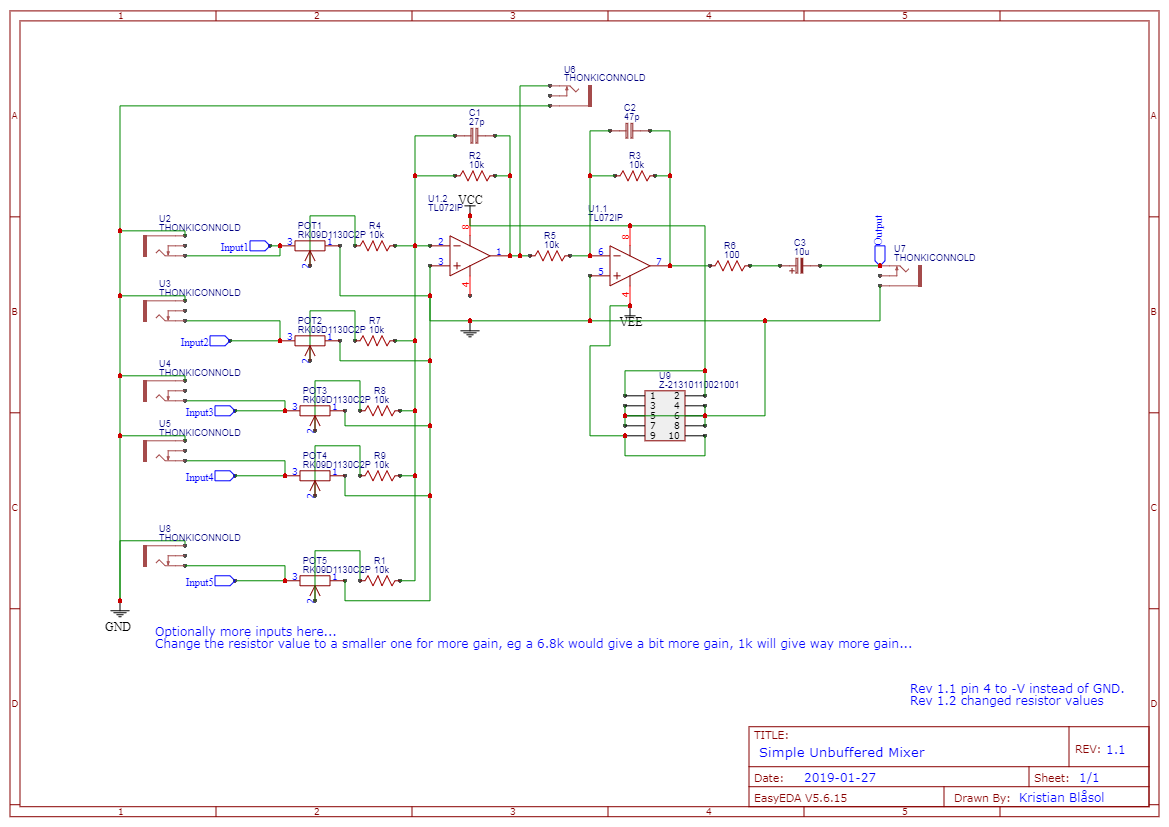
\includegraphics[width=.9\linewidth]{/home/felixp/Documents/diplomarbeit/dokumentation/figures/Schematic_Simple_Mixer.png}
\caption{Schaltkreis für einen passiven Mixer; Quelle: (Kristian Blåsol, 2018a)}
\end{figure}
\subsubsection{Benutzung}
\label{sec:orgfe7ece5}
Es können bis zu drei zu mixende Signale an die oberen Audiobuchsen angeschlossen werden. Die unteren beiden Audiobuchsen liefern das Ausgangssignal, wobei der rechte der invertierende Ausgang ist. Als einfachen Patch könnte man die beiden Signale des Oszillator-Moduls (siehe Abschnitt \ref{Osci}) zusammenführen, um beide Oszillatoren auf einmal zu hören.

\label{VCA}
\subsection{Spannungskontrollierter Verstärker}
\label{sec:orgfe23552}
Ein \acf{VCA} verstärkt ein angelegtes Signal um einen Faktor, welcher proportional zur angelegten \acl{CV} ist. \acp{VCA} sind essentiell, um den erzeugten Klängen einen Rhythmus zu verleihen, da ohne \ac{VCA} keine dynamische Lautstärkeänderung möglich ist. 
\subsubsection{Spezifikationen}
\label{sec:org33bbcce}
\subsubsection{Elektronik}
\label{sec:org8fd69de}
Es gibt eine Vielzahl von möglichen Ansätzen für die technische Umsetzung eines \ac{VCA}. Die simpelste Möglichkeit ist es wohl, eine Vactrol zu benutzen, da diese mit nur minimaler Beschaltung zu einem VCA umgewandelt werden kann todo: schematic einfügen:\url{https://www.dropbox.com/s/o6oiyanco8lzmvt/Schematic\_Vactrol.pdf?dl=0}. Jede Art von \ac{VCA} hat einen gewissen Eigenklang, wobei ein Vactrol-VCA eine sehr "`glatte"' Dynamik erzeugt. Abrupte Spannungsänderungen in der \acl{CV} werden geglättet, wodurch das ausgehende Signal nur eine stetige Änderung in der Lautstärke erfahren kann.

Ein weiterer Ansatz nutzt den linearen Reaktionsbereich zweier NPN-Transistoren, wobei durch die Beschaltung auf einem der Transistoren genau das gegenteilige Signal, allerdings mit dem gleichen positiven Offset erzeugt wird. Diese zwei Signale werden dann von einem Operationsverstärker voneinander abgezogen, wodurch der positive Offset eliminiert wird und das modulierte Signal übrig bleibt. Eine Vielzahl von selbstregelnden Rückkopplungsschleifen trägt dazu bei, dass diese Art von \ac{VCA} besonders stabil und schnell auf Änderungen in der angelegten Kontrollspannung reagieren kann.
\subsubsection{Schematics}
\label{sec:orgaa19a8d}
\subsubsection{Benutzung}
\label{sec:orgc570447}
\acp{VCA} können durch eine Vielzahl an Modulen angesteuert werden. Am häufigsten ist wohl eine Art von Hüllkurvengenerator, um die Lautstärkeänderung bei einem Tastenanschlag zu simulieren. Ein einfacheres Beispiel wäre eine Rechteckswelle von einem LFO, um eine Art Stakkato zu erzeugen, oder ein langsam schwingender Sinus für eine Art Wobbel-Effekt.

\label{AR}
\subsection{Attack-Release Hüllkurvengenerator}
\label{sec:orgb2f9ce6}
Hüllkurvengeneratoren sind Module, welche bei Eingang eines Gate-Signals eine Hüllkurve generieren. Diese kann beispielsweise dazu genutzt werden, einen \ac{VCA} anzusteuern, welcher einem Klang Rhythmus und Dynamik, also eine sich Ändernde Lautstärke verleiht. Aufgrund der Komplexität eines vollständigen \ac{ADSR} Hüllkurvengenerators haben wir uns dazu entschieden, einen simpleren \ac{AR} Hüllkurvengenerator zu bauen. Dieser besitzt einen Eingang für eine \acl{CV}, an welchen ein Gate-Signal angelegt werden kann und zwei Drehpotentiometer, mit denen die Parameter Attack und Release eingestellt werden können. Attack stellt dabei die Zeit dar, die das Signal nach dem Drücken einer Taste beziehungsweise nach dem Anfang eines eingehenden Gate-Signals benötigt, um seinen Maximalwert zu erreichen. Release stellt die Zeit dar, die die Spannung der Hüllkurve nach dem Schließen des Gates benötigt, um wieder \SI{0}{\volt} zu erreichen.

\subsubsection{Spezifikationen}
\label{sec:org35aa45b}
\subsubsection{Elektronik}
\label{sec:orgafb251b}
In unserer Umsetzung wird das Potential am Eingang für eine \acl{CV}, an welchem ein Gate-Signal erwartet wird, von einem Operationsverstärker auf 12V verstärkt. Durch den oberen Signalpfad füllt sich ein großer Kondensator. Die Spannung, welche am Kondensator anliegt, wird gleichzeitig von einem Spannungsfolger gepuffert, da diese auch die Ausgangsspannung darstellt. Wird das Gate geschlossen, fällt die Spannung über den unteren Signalpfad wieder ab. Durch die Potentiometer kann man die Geschwindigkeit dieser beiden Prozesse kontrollieren.
\subsubsection{Schematics}
\label{sec:orgfad6b53}
\begin{figure}[htbp]
\centering
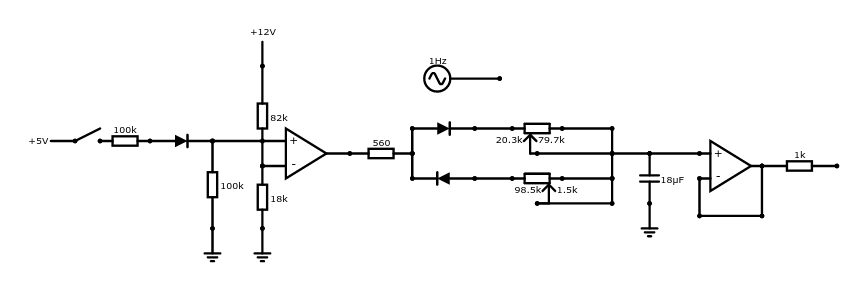
\includegraphics[width=.9\linewidth]{/home/felixp/Documents/diplomarbeit/dokumentation/figures/Schematic_AR.png}
\caption{Schaltkreis für einen simplen Attack Release Hüllkurvengenerator; Quelle: (Nathan Ramsden, 2016)}
\end{figure}
\subsubsection{Benutzung}
\label{sec:orgdacc2bc}
Unser AR bietet einen Eingang für Kontrollspannung vom Typ Gate, welcher angibt, ob etwa eine Taste gedrückt oder nicht. Außerdem ist ein Ausgang für die Hüllkurve vorhanden, welcher als \acl{CV} für einen \ac{VCA} vorhergesehen ist.


\appendix                       %% closes main document, appendix follows until end; only available in book-classes

\addpart*{Appendix}             %% adding Appendix to tableofcontents



% \begin{acronym}
% \acro{Kürzel}[Kurzform]{Langform}
% \end{acronym}

\chapter{Abkürzungsverzeichnis}

\begin{acronym}
  \acro{ADSR}[ADSR]{Attack, Decay, Sustain, Release}
  \acro{AR}[AR]{Attack-Release}
  \acro{CV}[CV]{Kontrollspannung}
  \acro{HE}[HE]{Höheneinheit}
  \acroplural{HE}[HE]{Höheneinheiten}
  \acro{LDR}[LDR]{Lichtabhängiger Widerstand, englisch: Light Dependent Resistor}
  \acro{LED}[LED]{Leuchtdiode, englisch: Light Emitting Diode}
  \acro{LFO}[LFO]{Oszillator mit niedriger Frequenz, englisch: Low Frequency Oscillator}
  \acro{THT}[THT]{Through Hole Technology}
  \acro{VCA}[VCA]{spannungskontrollierter Verstärker, englisch: Voltage Controlled Amplifier}
  \acro{VCF}[VCF]{spannungskontrollierter Filter, englisch: Voltage Controlled Filter}
  \acro{VCO}[VCO]{spannungskontrollierter Oszillator, englisch: Voltage Controlled Oscillator}
\end{acronym}

%\listoftables
\listoffigures
%\lstlistoflistings
\nocite{*} %Es werden auch nicht referenzierte Literaturstellen aufgelistet
\bibliography{references}

\end{document}
